\chapter{T2K and SK Experiment Overview}
\label{chap:T2KSKExp}

\finish{Event displays would be good}

\section{The Super-Kamiokande Experiment}
\label{sec:T2KSKExp_SK}

The SK experiment began taking data in 1996 \cite{Fukuda1998-tw} and has had many modifications throughout its lifespan. There has been six defined periods of data taking as noted in \autoref{tab:T2KSKExp_SKPeriods}. Between the SK-I and SK-II periods, a significant proportion of the PMTs were damaged during maintainence. Those that survived were equally distributed throughout the detector in the SK-II era, which resulted in a reduced photo-coverage. From SK-III onwards, significant repair efforts were made such that the full suite of PMTs were operational. Before the start of SK-IV, the data acquisition and electronic systems were upgraded. Between SK-IV and SK-V, a significant effort was placed into tank open maintainence and repair/replacement of defective PMTs, a task in which the author of this thesis was required for. Consequently, the detector conditions were significantly different between the two operational periods. SK-VI saw the start of the \quickmath{0.01\%} gadonlium doped water being introduced into the tank and the detector continues to operate to this day. Efforts are currently underway to increase the gadolinium concentrate in the likely start of the next SK period \finish{Link to Linyan's talk from Nu2022}.

\begin{table}[ht!]
    \centering
    \begin{tabular}{c|l|l|c}
      \hline
      Period & Start Date & End Date & Live-time (days) \\
      \hline
      I & April 1996 & July 2001 & 1489.19 \\
      II & October 2002 & October 2005 & 798.59 \\
      III & July 2006 & September 2008 & 518.08 \\
      IV & September 2008 & May 2018 & 3244.4 \\
      V & January 2019 & July 2020 & 461.02 \\
      VI & July 2020 & Ongoing & 583.3 \\
      \hline 
      \hline
    \end{tabular}
    \caption{The various SK periods and respective live-time. The SK-VI live-time is calculated until \quickmath{1^{\text{st}}} April 2022.}
    \label{tab:T2KSKExp_SKPeriods}
\end{table}

\subsection{The SK Detector}
\label{subsec:T2KSKExp_SKDetector}

The basic structure of the Super-Kamiokande (SK) detector is a cylindrical tank with diameter \quickmath{39.3\text{m}} and hieght \quickmath{41.1\text{m}} filled with ultrapure water \cite{Abe_2014_SKCalib}. A diagram of the signficant parts of the SK detector is illustrated in \autoref{fig:T2KSKExp_SK_Diag}. The SK detector is situated in the Kamioka mine in Gifu, Japan. The cavern in which the detector is located is underground with roughly \quickmath{1\text{km}} rock overburden (\quickmath{2.7 \text{km}} water equivalent overburden) \cite{Fukuda2003-ly}. At this depth, the rate of cosmic ray muons is significantly decreased to a value of \quickmath{\approx 2\text{Hz}}, compared to a surface-level detector. The top of the tank is covered with stainless steel which is designed as a working platform for maintainence, calibration and location for high voltage and data acquisition electronics.

\begin{figure}[h]
  \begin{subfigure}[t]{0.95\textwidth}
    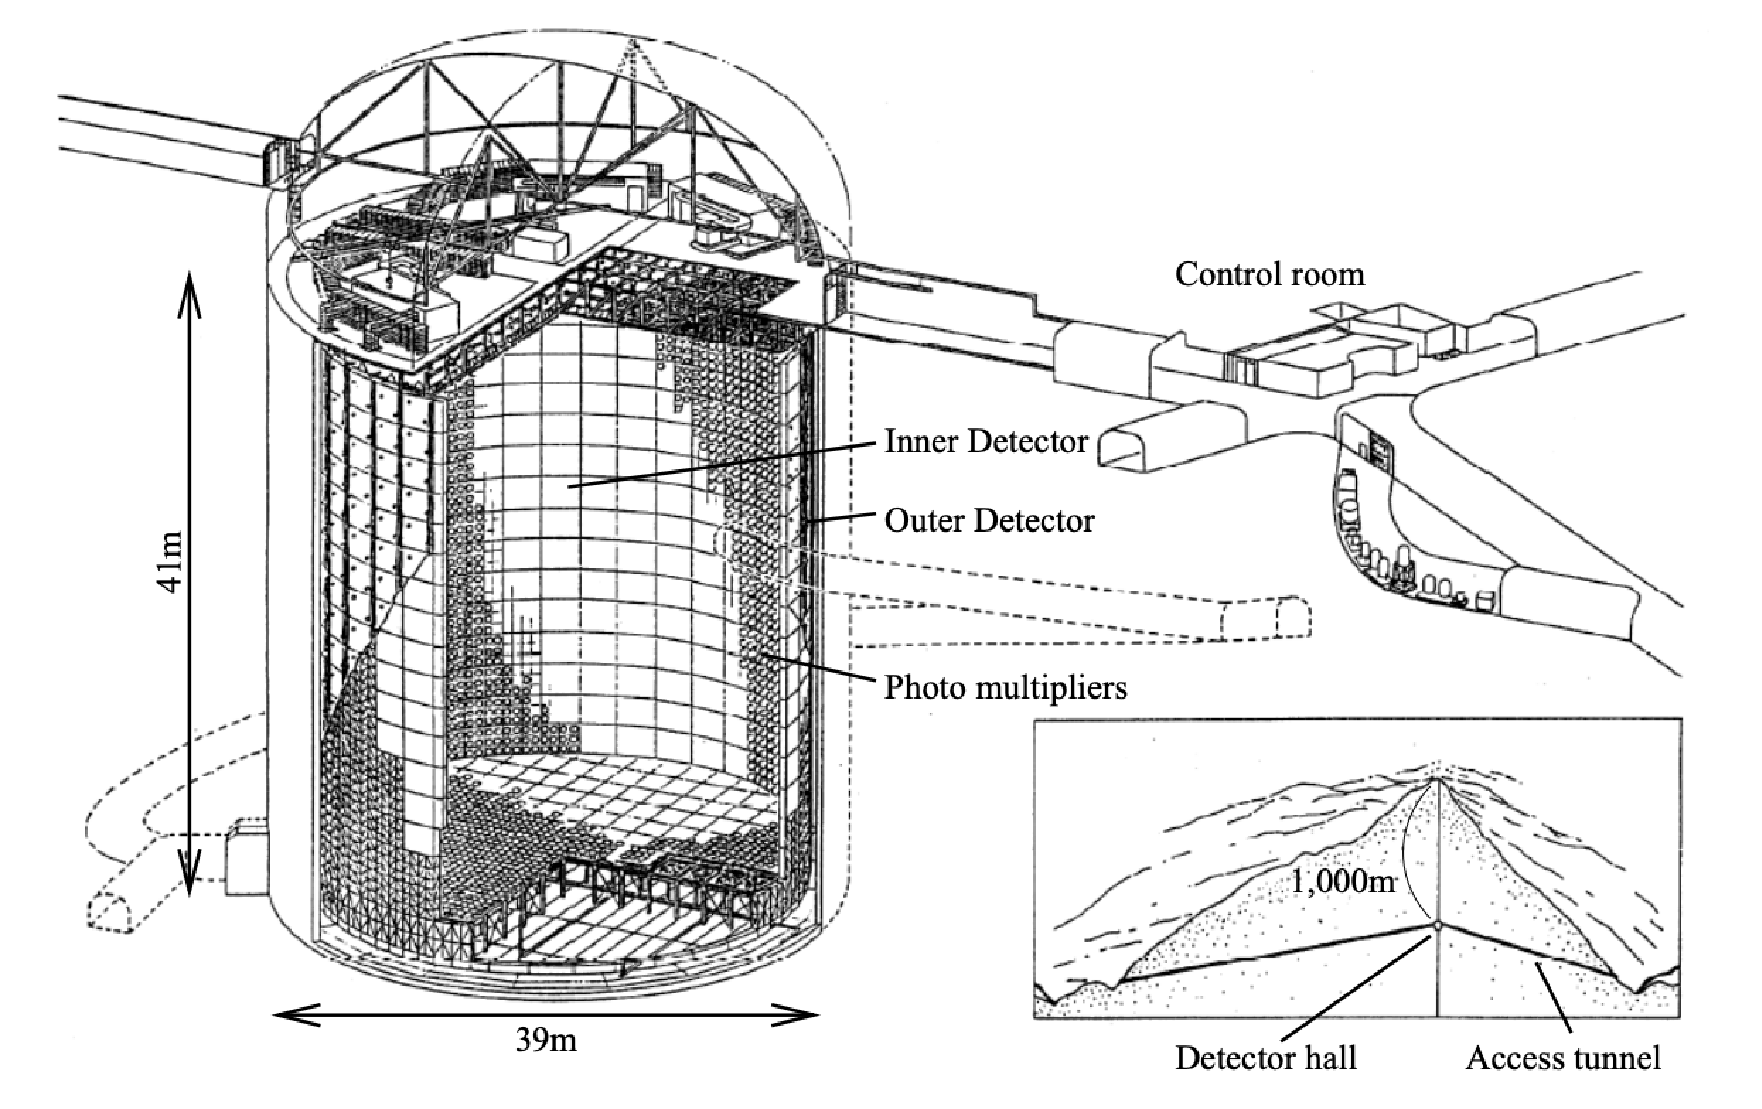
\includegraphics[width=\textwidth, trim={0mm 0mm 0mm 0mm}, clip,page=1]{Figures/Detectors/SKDiagram.pdf}
  \end{subfigure}
  \caption{A schematic diagram of the Super-Kamiokande Detector. Taken from \cite{Itow2001-bc}.}
  \label{fig:T2KSKExp_SK_Diag}
\end{figure}

A smaller cylindrical structure (\quickmath{36.2\text{m}} diameter, \quickmath{33.8\text{m}} hieght) is situated inside the tank, with an approximate \quickmath{2\text{m}} gap between this structure and the outer tank wall. The purpose of this structure is to support the photomultiplier tubes (PMTs). The volume inside and outside the support structure are referred to as the inner detector (ID) and outer detector (OD), respectively. In the SK-IV era, the ID and OD are instrumented by \quickmath{11129} \quickmath{50\text{cm}} and \quickmath{1885} \quickmath{20 \text{cm}} PMTs respectively \cite{Abe_2014_SKCalib}. The inner detector contains a \quickmath{32\text{kton}} volume of water, although many analyses performed at SK use a ``fiducial volume'' defined by the volume of water inside the ID excluding some distance to the ID wall. This reduces the volume of detector which is sensitive to neutrino events but reduces radioactive backgrounds and allows for better constraints on the reconstruction systematics. The nominal fiducial volume is defined as the area contained inside \quickmath{2\text{m}} from the ID wall for a total of \quickmath{22.5\text{kton}} water \cite{Jiang2019-iw}.

The two regions of the detector (ID and OD) are optically separated with opaque black plastic. The purpose of this is to deteremine whether a track entered or exited the ID. This allows cosmic muon rays and partially contained events to be tagged and separated from neutrino events entirely contained within the detector's sensitive region. This black plastic is also used to cover the area between the ID PMTs to reduce photon reflection from the ID walls. Contrary to this, the OD is lined with a reflective material (called Tyvek) to allow photons to reflect around inside the OD until collected by one of the PMTs. Furthermore, each OD PMT is backed with \quickmath{50\times50\text{cm}} plates of wavelength shifting acrylic which increases the efficiency of light collection \cite{Fukuda2003-ly}.

In the SK-IV data taking period, the photocathode coverage of the detector, or the fraction of the ID wall instrumented with PMTs, is \quickmath{\sim 40\%} \cite{Fukuda2003-ly}. The PMTs have a quantum efficiency (the ratio of detected electrons to incident photons) of \quickmath{\sim 21\%} for photons with wavelengths of \quickmath{360\text{nm} < \lambda < 390\text{nm}}. The proportion of photoelectrons which produce a signal in the dynode of a PMT, termed the collection efficiency, is \quickmath{>70 \%} \cite{Fukuda2003-ly}. The PMTs used within SK are most sensitive to photons with wavelength \quickmath{300\text{nm} \leq \lambda \leq 600\text{nm}} \cite{Fukuda2003-ly}. One disadvantage of using PMTs as the detection media is that the Earth's geomagnetic field can modify their response. Therefore, a set of compensation coils is built around the inner surface of the detector to mitigate this effect.

As mentioned, the SK detector is filled with ultrapure water, which in a perfect world would contain no impurities. However bacteria and organic compounds can significantly degrade the water quality, thus decreasing the attenuation length thus reducing the total number of photons which could be detected by the PMTs. To combat this, a sophisticated water treatment system has been developed \cite{Fukuda2003-ly, Nakano2020-sb}. UV lights, mechanical filters and membrane degasifiers are used to reduce the bacteria, suspended particulates and radioactive materials from the water. The flow of water within the tank is also critical as it can remove stagnant bacterial growth or build up of dust on the surfaces within the tank. Gravity drifts impurities in the water towards the bottom of the tank which if left uncontrolled, can create asymetric water conditions between the top and bottom of the tank.
%The flow of water in the tank can be controlled via mechanically driven circulation or temperature driven convection.
Typically, the water entering the tank is cooled below the ambient temperature of the tank to control convection and inhibit bacteria growth. Furthermore, the dark noise hits within PMTs is sensitive to the PMT temperature \cite{HamamatsuPMT} so controlling the temperature gradients within the tank is beneficial for stable measurements.

SK-VI is the first phase of the SK experiment to use gadonlium dopants within the ultrapure water \finish{Link to Linyan's talk at Nu2022}. As such, the SK water system had to be replaced to avoid removing the gadolium concentrate from the ultrapure water \cite{Abe2022-qq}. For an inverse \quickmath{\beta}-decay (IBD) interaction in a water target, the emitted neutron is thermally captured on hydrogen. This process releases \quickmath{2.2 \text{MeV}} \quickmath{\gamma} rays which are difficult to detect due to Compton scattered elecrtons from a \quickmath{\gamma} ray of this energy is very close to the Cherenkov threshold, limiting the number of photons produced. Thermal capture of neutrons on gadolinium generates \quickmath{\gamma} rays with higher energy meaning they are more easily detected. SK-VI has \quickmath{0.01 \%} Gd loading (\quickmath{0.02\%} gadolinium sulphate by mass) which causes \quickmath{\approx 50\%} of neutrons emitted by IBD to be captured on gadolinium \cite{PhysRevLett.93.171101,Marti2020-le} . Whilst predominantly useful for low energy analyses, Gd loading allows \quickmath{\nu/\bar{\nu}} separation for atmopsheric neutrino event selections \cite{Marti2019-gu}. Efforts are currently in place to increase the gadolinium concentrate to \quickmath{0.03 \%} for \quickmath{\approx 75\%} neutron capture efficiency on gadonlium \finish{Link to Mark's talk at Nu2022}. The final stage of loading targets \quickmath{0.1 \%} concentrate.

\subsection{Calibration}
\label{subsec:T2KSKExp_SKCalibration}

The calibration of the SK detector is documented in \cite{Abe_2014_SKCalib} and summarised below. The analysis presented within this thesis is dependent upon `high energy events' (Charged particles with \quickmath{O(>100)\text{MeV}} momenta). These are events which are expected to generate a larger number photons such that each PMT will be hit with multiple photons. The reconstruction of these events depends upon the charge deposited within each PMT and the timing response of each individual PMT. Therefore, the most relevent calibration techniques to this thesis are outlined.

Before installation, \quickmath{420} PMTs were calibrated to have identical charge response and then distributed throughout the tank in a cross-shape pattern (As illustrated by \autoref{fig:T2KSKExp_SK_StandardPMTs}). These are used as a standardised measure for the rest of the PMTs installed at similar geometric positions within SK to be calibrated against. This allows each PMT to have it's high voltage set so that all PMTs give the same signal for an identical light collection. To perform this calibration, a xenon lamp is located at the center of the SK tank which flashes uniform light at \quickmath{1 \text{Hz}}. This allows for geometrical effects, water quality variation and timing effects to be measured in-situ throughout normal data taking periods.

\begin{figure}[h]
  \begin{subfigure}[t]{0.50\textwidth}
    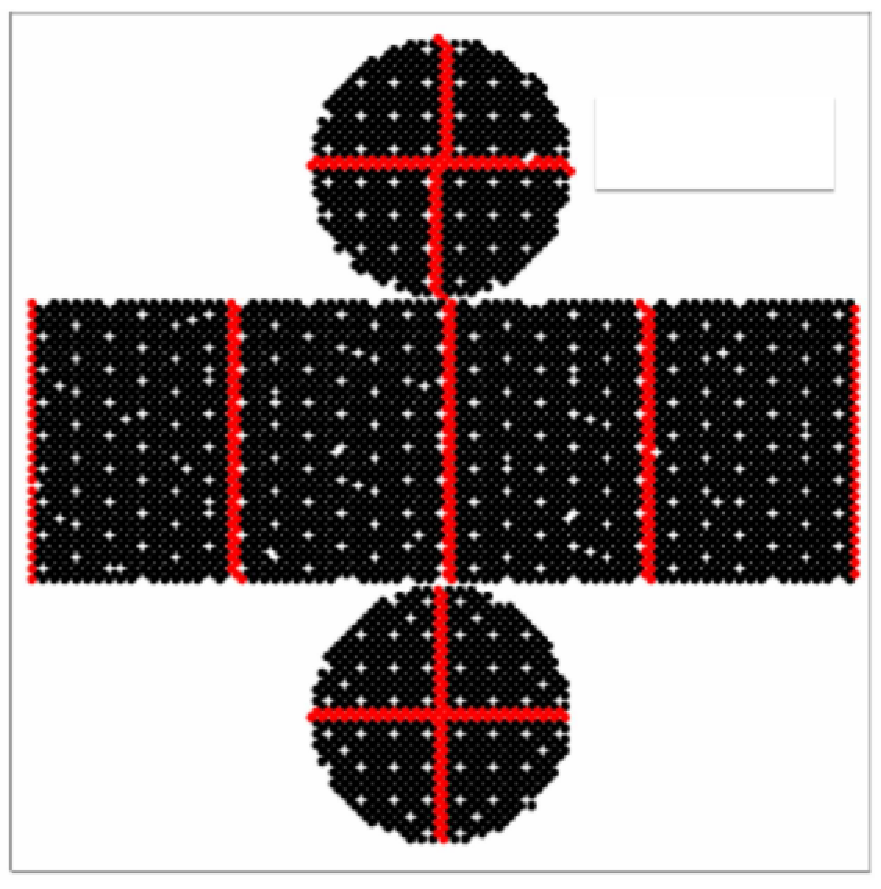
\includegraphics[width=\textwidth, trim={0mm 0mm 0mm 0mm}, clip,page=1]{Figures/Detectors/StandardPMTs.pdf}
  \end{subfigure}
  \caption{The location of ``standard PMTs'' (red) inside the SK detector. Taken from \cite{Abe_2014_SKCalib}.}
  \label{fig:T2KSKExp_SK_StandardPMTs}
\end{figure}

When specifically performing calibration of the detector (in out-of-data taking mode), the water in the tank was circulated to avoid top/bottom asymmetric water quality. Any non-uniformity within the tank significantly effects the PMT hit probability through scattering or absorption. This becomes a dominant effect for the very low intensity light sources discussed later which are designed such that only one photon is incident upon a given PMT.

The ``gain'' of a PMT is defined as the ratio of total charge of the signal produced compared to the charge of photoelectrons emitted by the photocathodes within the PMT. To calibrate the signal of each PMT, the ``relative'' and ``absolute'' gain values are measured. The relative gain is the variation of gain among each of the PMTs whereas the absolute gain is the average gain of all PMTs. 

The relative gain is calibrated as follows. A laser light is used to generate measurements under two conditions; a high-intensity flash which illuminates every PMT with a sufficient number of photons, and a low-intensity flash in which only a small number of PMTs collect light. The first measurement creates an average charge, \quickmath{Q_{obs}(i)} on PMT \quickmath{i}, whereas the second measurement ensures that each hit PMT only generates a single photoelectron. For the low intensity measurement, the number of times each PMT records a charge larger than \quickmath{1/4} photoelectrons, \quickmath{N_{obs}(i)} is counted. The values measured can be expressed as

\begin{equation}
  \label{eq:T2KSKExp_RelativeGainCalib}
  \begin{split}
    Q_{obs}(i) &\propto I_{H} \times f(i) \times \epsilon(i) \times G(i), \\
    N_{obs}(i) &\propto I_{L} \times f(i) \times \epsilon(i),
  \end{split}
\end{equation}

Where \quickmath{I_{H}} and \quickmath{I_{L}} is the intensity of the high and low flashes, \quickmath{f(i)} is the acceptance efficiency of the \quickmath{i^{\text{th}}} PMT, \quickmath{\epsilon(i)} is the product of the quantum and collection efficiency of the \quickmath{i^{\text{th}}} PMT and \quickmath{G(i)} is the gain of the \quickmath{i^{\text{th}}}	PMT. The relative gain for each PMT can determined by taking the ratio of these quantities.

The absolute gain calibration is performed by observing fixed energy \quickmath{\gamma}-rays of \quickmath{E_{\gamma} \approx 9\text{MeV}} emitted isotropically from neutron capture on a NiCf source situated at the centre of the detector. This generates a photon yeild of about \quickmath{0.004} photoelectrons/PMT/event, meaning that \quickmath{>99\%} of PMT signals are generated from a single photoelectron. A charge distribution is generated by performing this calibration over all PMTs, and the average value of this distribution is taken to be the absolute gain value. It has been found that the absolute gain increases as a function of time despite there being no known reason for this behaviour.

As mentioned in \autoref{subsec:T2KSKExp_SKDetector}, the average quantum and collection efficiency for the SK detector is \quickmath{\sim 21\%} and \quickmath{>70 \%} respectively. However, these values do differ between each PMT and need to be calibrated accordingly. Consequently, the NiCf source is also used to calibrate the ``quantum \quickmath{\times} collection'' efficiency (denoted ``QE'') value of each PMT. This value is calculated as calibrating the signal generated by one incident photon is of more importance than the individual efficiency of photoelectron emission or detection on the dynode. The NiCf low intensity source is used as the PMT hit probability is proportional to the QE (\quickmath{N_{obs}(i) \propto \epsilon(i)} in \autoref{eq:T2KSKExp_RelativeGainCalib}). A Monte Carlo prediction which includes photon absorption, scattering and reflection is made to estimate the number of photons incident on each PMT and the ratio of the number of predicted to observed hits is calculated. The difference is attributed to the QE efficiency of that PMT. This technique is extended to calculate the relative QE efficiency by normalizing the average of all PMTs which removes the dependence of the light intensity.

Due to differering cable lengths and readout electronics, the timing response between a photon hitting the PMT and the signal being captured by the data acquisition can be different between each PMT. Due to threshold triggers (Described in \autoref{subsec:T2KSKExp_SKTriggering}), the time at which a pulse reaches a threshold is dependent upon the size of the pulse. This is known as the `time-walk' effect and also needs to be accounted for in each PMT. To calibrate the timing response, a pulse of light with width \quickmath{0.2\text{nsec}} is emitted into the detector through a diffuser and observed by an external PMT which is used to measure the pulse start time. Two dimensional distributions of time and pulse height (or charge) are made for each PMT and are used to calibrate the timing response. This is performed in-situ whilst data taking with the light source pulsing at \quickmath{0.03\text{Hz}}.

The top/bottom water quality asymmetry is measured using the NiCf calibration data and cross-referencing these results to the ``standard PMTs''. The water attenuation length is continously measured by the rate of vertically-downgoing cosmic-ray muons which enter via the top of the tank.

In the ultra-relativistic approximation that \quickmath{\beta=1}, a charged particle will generate Cherenkov photons with a characteristic pitch angle of \quickmath{42^{\circ}}. By calculating the ratio of the charge deposited on PMTs within this cone angle to that outside of the cone, the rate of photon scattering can be calculated. This value is dependent upon the water quality inside the tank. Performing this calculation using cosmic ray muons allows the water quality to be monitored in real time. A more complex analysis, which uses a collimated laser to inject photons at different wavelengths is performed to determine the Rayleigh scattering, Mie scattering and absorption coefficients. This methodology divides the tank into five horizontal slices, where the timing and spatial distribution of hits PMTs in each slice can be compared between data and various Monte Carlo predictions. The coefficients which minimise the \quickmath{\chi^2} between data and Monte Carlo are selected and utilised within the detector simulation. 

\subsection{Data Acquisition and Triggering}
\label{subsec:T2KSKExp_SKTriggering}

Dark noise is the phenomenon where a PMT registers a pulse that is consistent with a single photoelectron emitted from photon detection despite being the PMT being in complete darkness. This is predominately caused by two processes. Firstly there is intrinsic dark noise which is where photoelectrons gain enough thermal energy to be emitted from the photocathode, and secondly, the radioative decay of contaminants inside the structure of the PMT which mimics the same effect. Typical dark noise rate for PMTs used within SK are \quickmath{O(3)\text{kHz}} \cite{Fukuda2003-ly} which equates to about \quickmath{12} dark noise hits per \quickmath{220\text{ns}} \cite{Carminati2015-zx}. This is lower than the expected number of photons generated for a `high energy event' (As described in \autoref{subsec:T2KSKExp_Cherenkov}) but instability in this value can cause biases in reconstruction.

The maximum distance that a photon can travel within the SK detector is \quickmath{\sim 200\text{ns}} \cite{PhysRevD.73.112001}. The earlier data acquisition and triggering systems are documented in \cite{34489,PhysRevD.73.112001}. The analysis presented in this thesis only uses the SK-IV period of the SK experiment so this subsection focuses on the relevant points of the data acquisition and triggering systems to that SK period.

Before the SK-IV period started, the existing front-end electronics were replaced with ``QTC-Based Electrons with Ethernet, QBEE'' systems \cite{Nishino2009-wh}. When the QBEE observes a signal above a \quickmath{1/4} photoelectron threshold, the charge-to-time (QTC) converter generates a rectangular pulse. The start of the rectangular pulse indicates the time at which the analogue photoelectron signal was recieved and the width of the pulse indicates the total charge intergrated throughout the signal. This is then digitized by time-to-digital converters and sent to the ``front-end'' PCs. The digitized signal from every QBEE is then chronologically order and sent to the ``merger'' PCs. It is the merger PCs which apply the software trigger and send any `interesting' events the ``organizer'' PC. This sorts the data stream of multiple merger PCs into chrolonolgically ordered events in time which is then saved to disk. The schematic of data flow from PMTs to disk is illustrated in \autoref{fig:T2KSKExp_SK_DataFlow}.

\begin{figure}[h]
  \begin{subfigure}[t]{0.80\textwidth}
    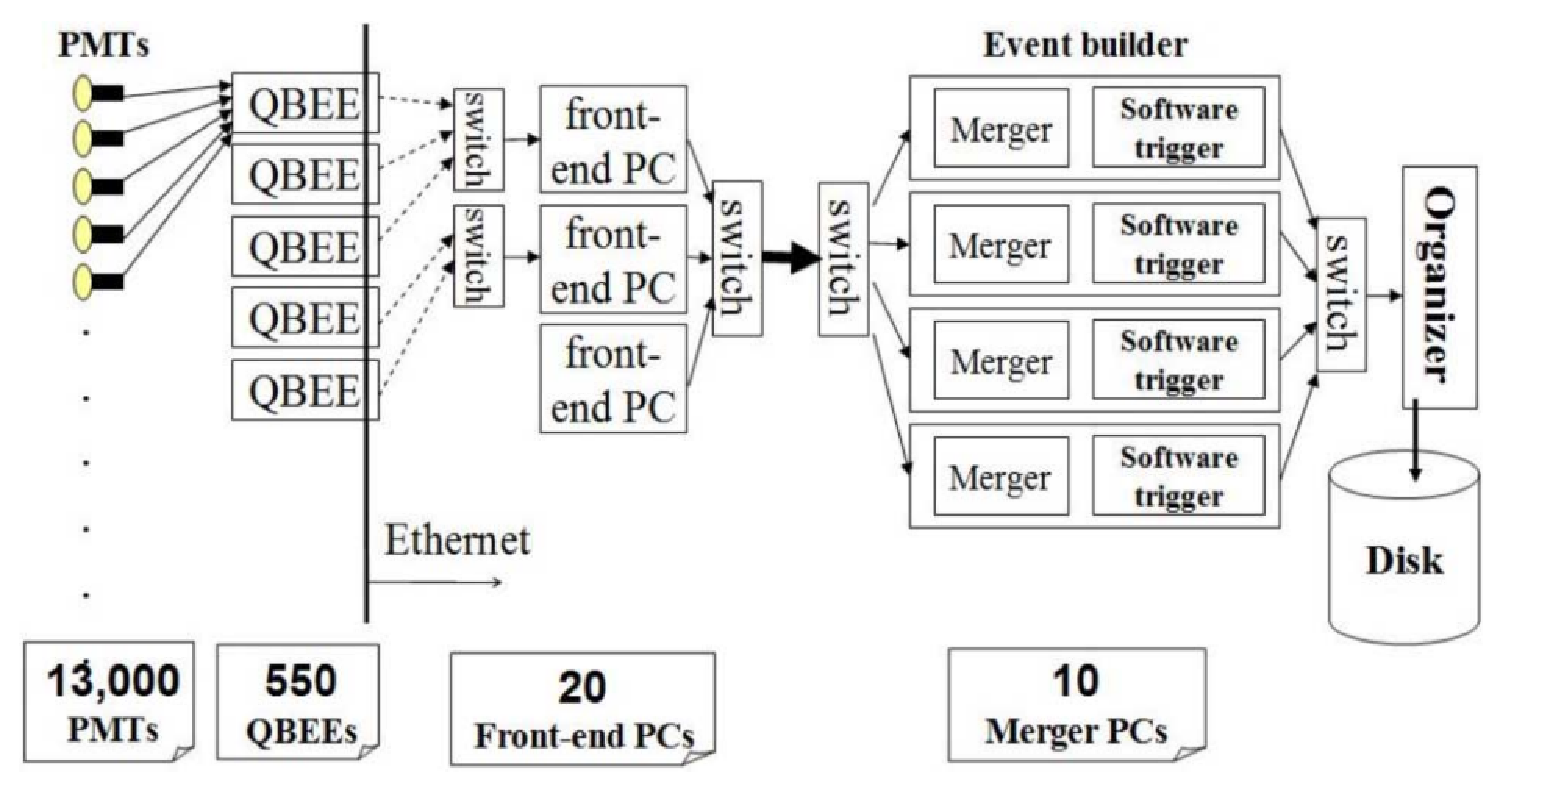
\includegraphics[width=\textwidth, trim={0mm 0mm 0mm 0mm}, clip,page=1]{Figures/Detectors/SKDataFlow.pdf}
  \end{subfigure}
  \caption{Schematic view of the data flow through the data acquistion and online system. Taken from \cite{5446533}.}
  \label{fig:T2KSKExp_SK_DataFlow}
\end{figure}

%The software trigger applied in SK-IV replaces the hardware trigger applied in SK-I to SK-III.
The software trigger (described in \cite{Yamada2007-cp}) operates by determining the number of PMT hits within a \quickmath{200\text{ns}} sliding window, \quickmath{N_{200}}, which coincides with the maximum time that a Cherenkov photon would take to traverse the length of the SK tank. For lower energy events which generate fewer photons, this technique is useful for eliminating background processes like dark noise and radioactive decay which would be expected to separated in time. When the value of \quickmath{N_{200}} exceeds some threshold, a software trigger is issued. There are several trigger thresholds used within the SK-IV period which are detailed in \autoref{tab:T2KSKExp_TriggerThreshold}. If one of these thresholds is met, the PMT hits within an extended time window is also readout and saved to disk. The length of the time window is also included in the tabulated threshold conditions. In the special case of an event which exceeds the SHE trigger but does not exceed the OD trigger, the AFT trigger looks for delayed coincidences of \quickmath{2.2 \text{MeV}} gamma rays emitted from neutron capture in a \quickmath{535 \mu\text{s}} window after the SHE trigger. A similar but more complex ``Wideband Intelligent Trigger (WIT)'' has been deployed and is described in \cite{Carminati2015-zx}.

\begin{table}[ht!]
    \centering
    \begin{tabular}{l|c|c|c}
      \hline
      Trigger & Acronym & Condition & Extended time window (\quickmath{\mu \text{s}}) \\
      \hline
      Super Low Energy & SLE & >34/31 hits & 1.3 \\
      Low Energy & LE & >47 hits & 40 \\
      High Energy & HE & >50 hits & 40 \\
      Super High Energy & SHE & >70/58 hits & 40 \\
      Outer Detector & OD & >22 hits in OD & N/A \\
      \hline
      \hline
    \end{tabular}
    \caption{The trigger thresholds and extended time windows saved around an event which were utilised throughout the SK-IV period. The exact thresholds can change and the values listed here represent the thresholds at the start and end of the SK-IV period.}
    \label{tab:T2KSKExp_TriggerThreshold}
\end{table}

\subsection{Cherenkov Radiation}
\label{subsec:T2KSKExp_Cherenkov}

Cherenkov light is emitted from any highly energetic charged particle travelling with relativistic velocity \quickmath{\beta} greater than the local speed of light in a medium with refractive index \quickmath{n>1.0} \cite{Cerenkov1937-tl}. This occurs due to the charged particle exciting the polarised media, which de-excites via photon emission. From Huygen's principal, the emitted waves propagate outwards but only generate coherent wavefronts when the charged particle moves faster than the phase velocity of that media. Consequently, Cherenkov light is formed at the surface of a cone with characteristic pitch angle,

\begin{equation}
  \label{eq:T2KSKExp_CherenkovConeAngle}
  \cos(\theta)=\frac{1}{\beta n}.
\end{equation}

Consequently, the Cherenkov momentum threshold (where the requirement is \quickmath{\beta = 1/n}) is dependent upon the mass, \quickmath{m}, of the charged particle moving through the media,

\begin{equation}
  P_{thres} = \frac{m}{\sqrt{n^{2}-1}}
\end{equation}

For water, where \quickmath{n = 1.33}, the Cherenkov threshold momentum and energy for various particles is given in \autoref{tab:T2KSKExp_CherenkovThreshold}. In contrast, \quickmath{\gamma}-rays are directed indirectly via the combination of photons generated by compton scattering and pair production. The threshold for detection in the SK detector is typically higher than the threshold for photon production. This is due to the fact that the attenuation of photons in the water means that typically \quickmath{\sim 75\%} of Cherenkov photons reach the ID PMTs. Then the collection and quantum efficiencies described in \autoref{subsec:T2KSKExp_SKDetector} results in the number of detected photons being lower than the number of photons which reach the PMTs. 

\begin{table}[ht!]
    \centering
    \begin{tabular}{l|c|c}
      \hline
      Particle & Threshold Momentum (MeV) & Threshold Energy (MeV)\\
      \hline
      Electron & 0.5828 & 0.7751 \\
      Muon & 120.5 & 160.3 \\
      Pion & 159.2 & 211.7 \\
      Proton & 1070.0 & 1423.1 \\
      \hline
      \hline
    \end{tabular}
    \caption{The threshold momentum and energy for a particle to generate Cherenkov light in ultrapure water, as calculated in \autoref{eq:T2KSKExp_CherenkovConeAngle} in ultrapure water where \quickmath{n = 1.33}.}
    \label{tab:T2KSKExp_CherenkovThreshold}
\end{table}

The Frank-Tamm equation \cite{Frank1991-wj} describes the relationship between the number of Cherenkov photons generated per unit length, \quickmath{dN/dx}, the wavelength of the photons generated, \quickmath{\lambda} and the relativistic velocity of the charged particle,

\begin{equation}
  \label{eq:T2KSKExp_FrankTammFormula}
  \frac{d^2N}{dxd\lambda} = 2\pi\alpha \left(1 - \frac{1}{n^2 \beta^2} \right)\frac{1}{\lambda^2} .
\end{equation}

where \quickmath{\alpha} is the fine structure constant. For a \quickmath{100\text{MeV}} electron, approximately \quickmath{330} photons will be produced per centimeter in the \quickmath{300\text{nm} \leq \lambda \leq 700\text{nm}} region which the ID PMTs are most sensitive to \cite{Fukuda2003-ly}.

\finish{Plot of muon momentum showing difference between Cherenkov threshold and detected threshold}

\section{The Tokai to Kamioka Experiment}
\label{sec:T2KSKExp_T2K}

The Tokai to Kamioka (T2K) experiment is a long baseline neutrino oscillation experiment located in Japan. Proposed in the early 2000's \cite{jhf_loi, Itow2001-vw} as the replacement of K2K \cite{The_K2K_Collaboration2001-oo}, T2K was designed to observe electron neutrino appearance whilst precisely measuring the oscillation parameters associated with muon neutrino disappearance \cite{t2k_proposal}. The experiment consists of a neutrino beam generated at the Japan Proton Accelerator Research Complex (J-PARC), a suite of near detectors situated \quickmath{280\text{m}} from the beam target and the Super Kamiokande far detector positioned with a \quickmath{295\text{km}} baseline which observes the oscillated neutrino flux. The cross-section view of the T2K experiment is drawn in \autoref{fig:T2KSKExp_T2K_Overview}.

\begin{figure}[h]
  \begin{subfigure}[t]{0.95\textwidth}
    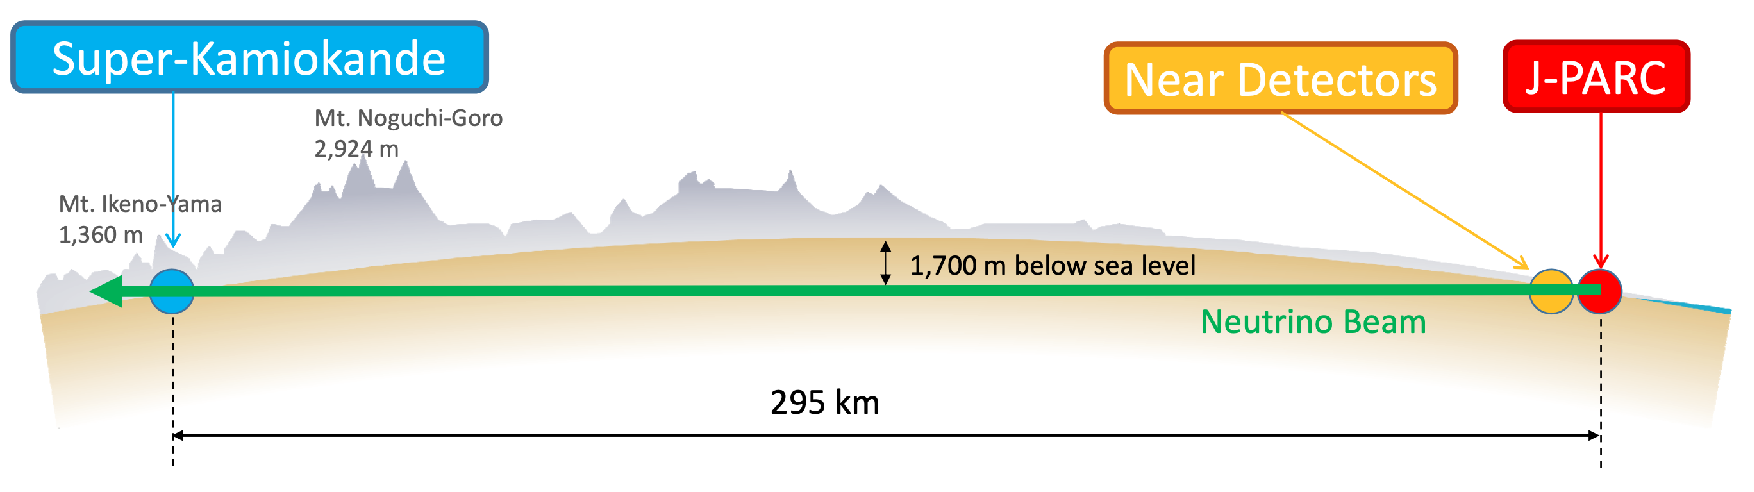
\includegraphics[width=\textwidth, trim={0mm 0mm 0mm 0mm}, clip,page=1]{Figures/Detectors/T2KCrossSection.pdf}
  \end{subfigure}
  \caption{The cross section of the Tokai to Kamioka experiment, illustrating the beam generation facility at J-PARC, the near detector situated at a baseline of \quickmath{280\text{m}} and the far detector situated \quickmath{295\text{km}} from the beam target.}
  \label{fig:T2KSKExp_T2K_Overview}
\end{figure}

The T2K collaboration make world leading measurements of the \sinsqatm, \delmsqatm and \dcp oscillation parameters and still keep improving their precision by including new samples and developing the models which describe the neutrino interactions and detector responses \finish{Link to Christophe's slides from Nu2022}. Electron neutrino appearance was first observed at T2K in 2014 \cite{2014_Abe_ElectronNuApp} which accompanied a \quickmath{7.3\sigma} significance of a non-zero \sinsqreac measurement.

The purpose of the near detectors is to constrain the beam flux and cross section model parameters used within the fit. This is because the neutrinos which the near detectors observe have not travelled a distance far enough for the oscillation probability to have significantly changed the neutrino flavour eigenstates from that of the generated neutrino beam. There are a host of detectors situated in the near detector hall (As illustrated in \autoref{fig:T2KSKExp_T2K_ND280Pit}); nd280 (\autoref{subsec:T2KSKExp_T2K_ND280}), INGRID (\autoref{subsec:T2KSKExp_T2K_INGRID}), NINJA \cite{ninja}, WAGASCI \cite{wagasci} and Baby-MIND \cite{baby_mind}. The latter three are not currently used within the oscillation analysis presented within this thesis.

\begin{figure}[h]
  \begin{subfigure}[t]{0.6\textwidth}
    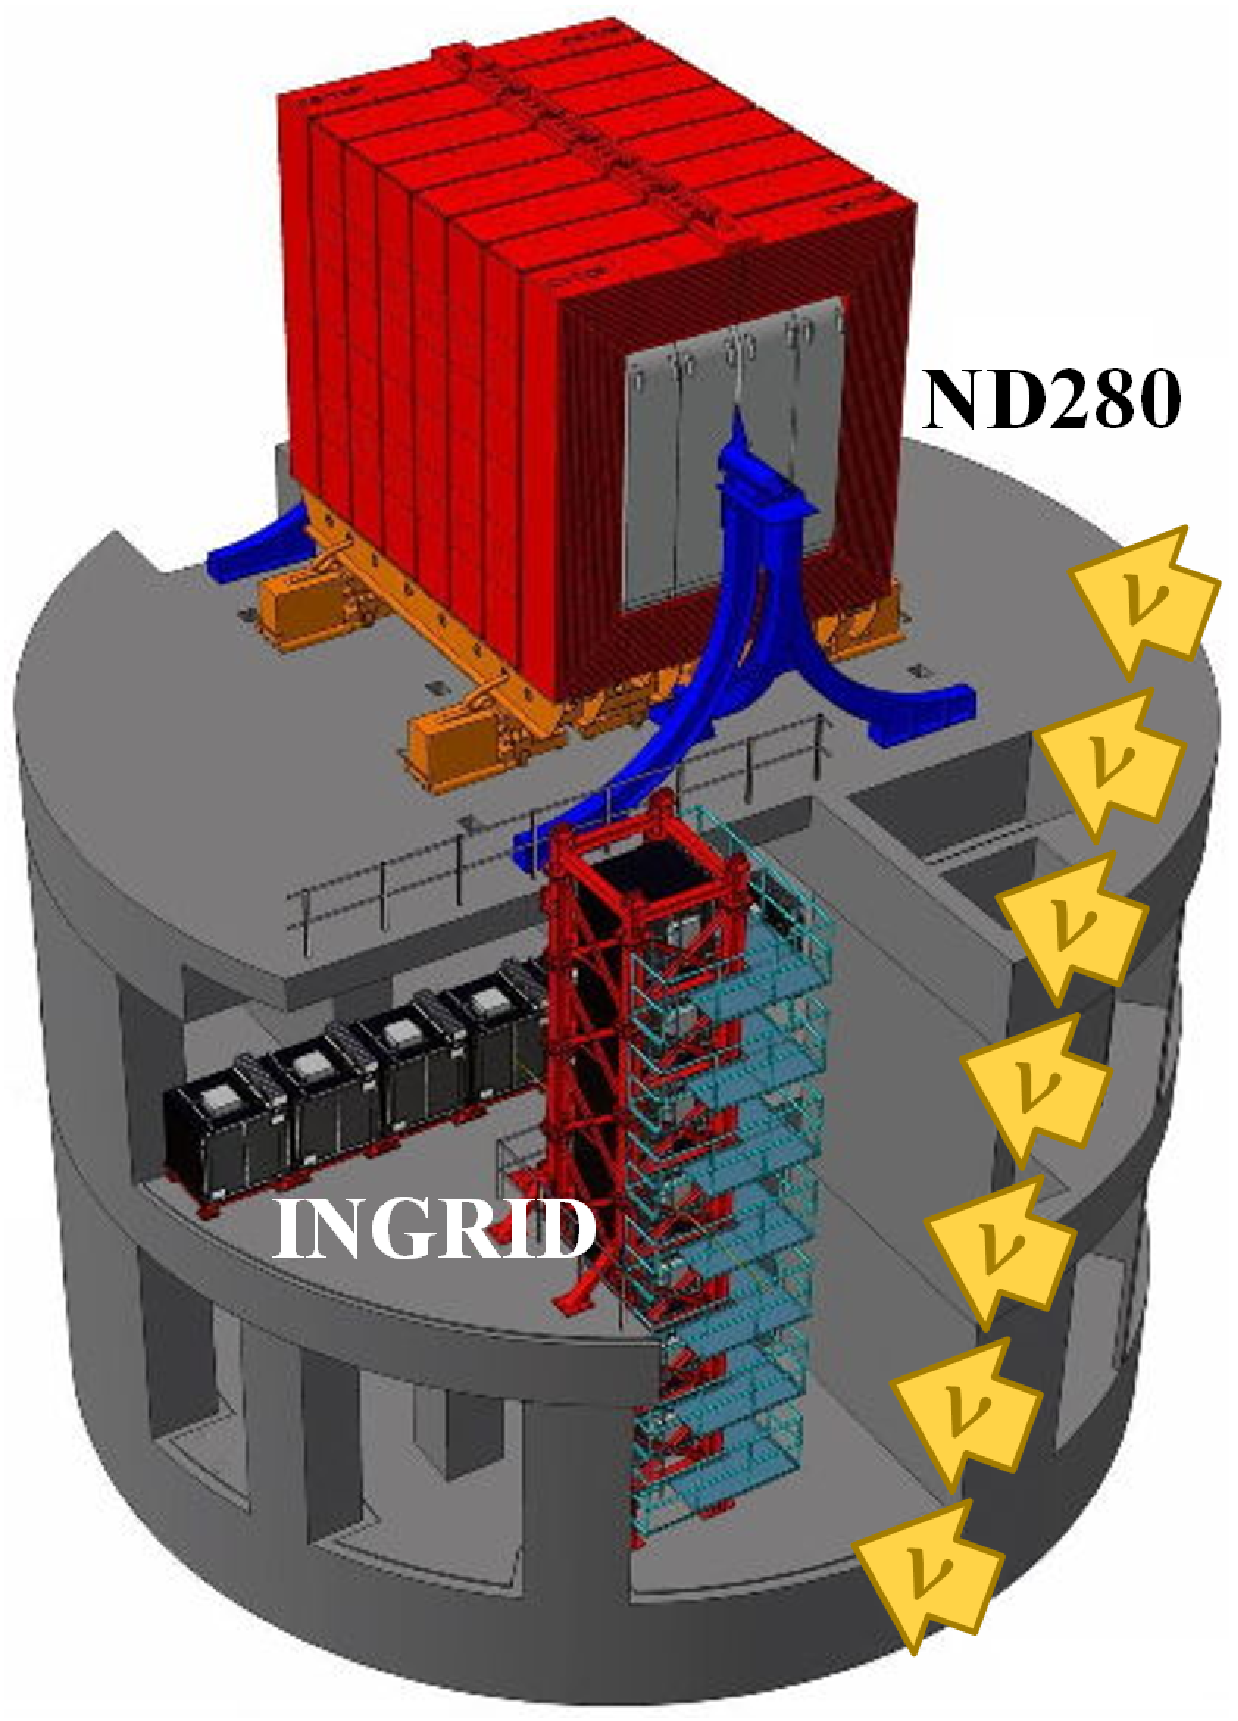
\includegraphics[width=\textwidth, trim={0mm 0mm 0mm 0mm}, clip,page=1]{Figures/Detectors/T2KND280Hall.pdf}
  \end{subfigure}
  \caption{The near detector suite for the T2K experiment. The distance between the detectors and the beam target is \quickmath{280\text{m}}.}
  \label{fig:T2KSKExp_T2K_ND280Pit}
\end{figure}

Whilst the purpose of ND280 described here is for the oscillation analysis, the detector can also make many cross section measurements for different interaction modes at neutrino energies of \quickmath{O(1)\text{GeV}} on the different targets within the detector \cite{PhysRevD.102.012007,10.1093/ptep/ptab014} . These measurements are of equal importance as they can lead the way in determining the model parameters used in the interaction models for the future high-precision era of neutrino physics.

\subsection{The Neutrino Beam}
\label{subsec:T2KSKExp_T2K_NeutrinoBeam}

The neutrino beam used within the T2K experiment is described in \cite{t2k_det, Abe_2013} and summarised below. The accelerating facility at J-PARC is composed of two sections; the primary and secondary beamlines. \autoref{fig:T2KSKExp_T2K_Beamline} illustrates a schematic of the beamline, focusing mostly on the components of the secondary beamline. The primary beamline has three accelerators which progressively accelerated protons; a linear accelerator, a rapid-cycling synchrotron and the main-ring (MR) synchrotron. Once fully accelerated by the MR, the proton's have a kinetic energy of \quickmath{30\text{GeV}}. Eigth bunches of these protons, separated by \quickmath{500\text{ns}}, are extracted per ``spill'' from the MR and directed towards a graphite target (A rod of length \quickmath{91.4\text{cm}} and diameter \quickmath{2.6\text{cm}}. A total of \quickmath{\sim 3\times 10^{14}} protons are contained in each spill. The rate of extracted spills is \quickmath{\sim 0.5\text{Hz}} although the width of the spill is \quickmath{\sim 5 \mu\text{s}}.

\begin{figure}[h]
  \begin{subfigure}[t]{0.7\textwidth}
    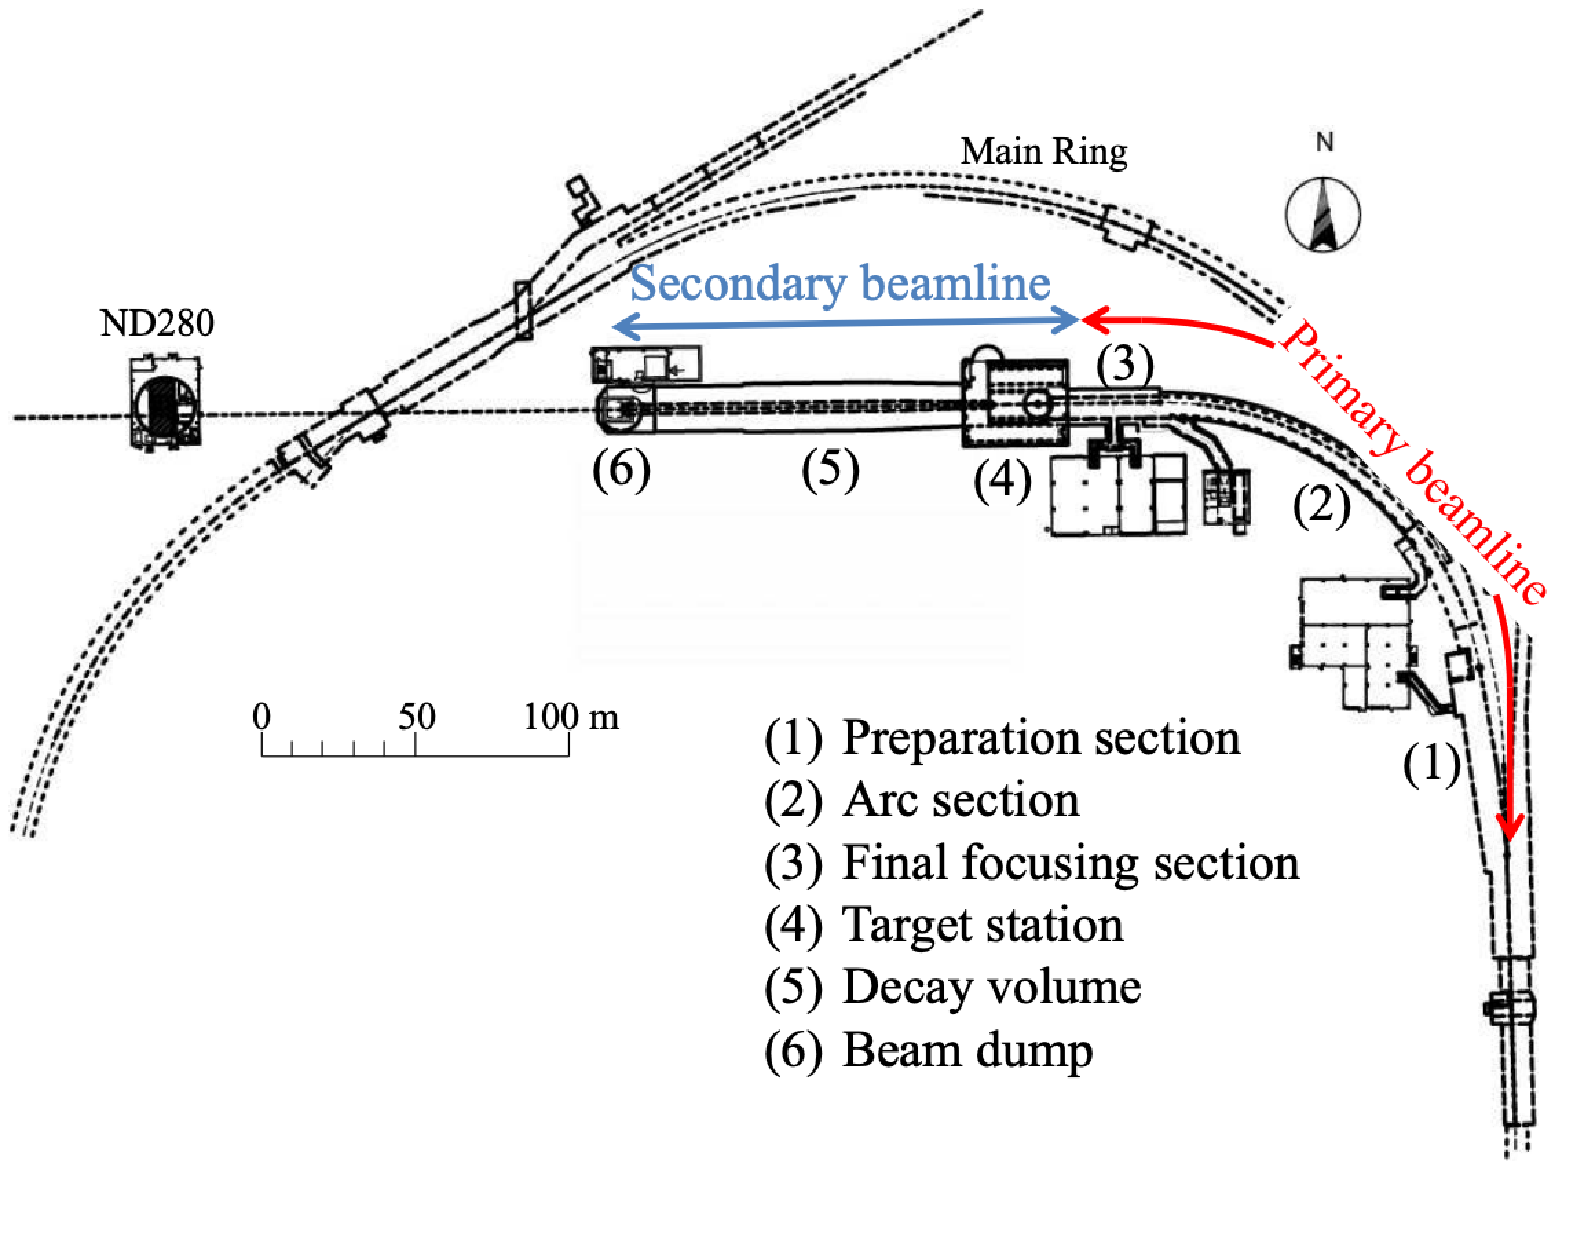
\includegraphics[width=\textwidth, trim={0mm 0mm 0mm 0mm}, clip,page=1]{Figures/Detectors/T2KBeamline.pdf}
    \subcaption{Primary and secondary beamline}
  \end{subfigure}
  \begin{subfigure}[t]{0.95\textwidth}
    \vspace{0.5cm}
    \includegraphics[width=\textwidth, trim={0mm 0mm 0mm 0mm}, clip,page=1]{Figures/Detectors/T2KSecondaryBeamline.jpg}
    \subcaption{Secondary beamline}
  \end{subfigure}
  \caption{Top figure: Bird's eye view of the most relevant part of primary and secondary beamline used within the T2K experiment. The primary beamline is the main-ring proton synchrotron, kicker magnet and graphite target. The secondary beamline consists of the the focusing horns, decay volume and beam dump. Figure taken from \cite{t2k_det}. Bottom figure: The side-view of the secondary beamline including the focusing horns, beam dump and neutrino detectors. Figure taken from \cite{MuMon}.}
  \label{fig:T2KSKExp_T2K_Beamline}
\end{figure}

The secondary beamline consists of three main components; the target station, the decay volume and the beam dump. The target station contains the target, beam monitors and three magnetic focusing horns. After the proton beam interacts with the graphite target, a host of particles emanates from the interaction vertex. This secondary beam is mostly composed of the pions and kaons, where the electrically charged component of the secondary beam is directed towards the far detector by the three magnetic focusing horns. These horns direct charged particles of a particular polarity towards SK whilst defocusing the oppositely charged particles. This allows a mostly neutrino or mostly antineutrino beam to be used within the experiment, denoted as ``forward horn current (FHC)'' or ``reverse horn current (RHC)'' respectively.

The focused beam of charged particles travels through a \quickmath{96\text{m}} long decay volume, generating a neutrino beam through the following decays \cite{Abe_2013},

\begin{equation}
  \begin{split}
    \pi^+ &\rightarrow \mu^+ + \nu_\mu \\
    K^+ &\rightarrow \mu^+ + \nu_\mu \\
    &\rightarrow \pi^0 + e^+ + \nu_e \\
    &\rightarrow \pi^0 + \mu^+ + \nu_\mu \\
    K^0_L &\rightarrow \pi^- + e^+ + \nu_e \\
    &\rightarrow \pi^- + \mu^+ + \nu_\mu \\
    \mu^+ &\rightarrow e^+ + \bar{\nu}_\mu + \nu_e
  \end{split}
\end{equation}

For low(high) neutrino energies, \quickmath{E_\nu < 3\text{GeV}}(\quickmath{E_\nu > 3\text{GeV}}), the \quickmath{\nu_\mu} component of the beam is dominanted by the pion(kaon) decay. The intrinsic \quickmath{\nu_e} contributions are dominated by muon decay for \quickmath{E_\nu < 2\text{GeV}} and by kaon decays above that energy. The ``wrong-sign'' component of the neutrino beam (the \quickmath{\bar{\nu}_\mu} component of the beam when operating in neutrino (FHC) mode or vice versa) is particularly prominent in th RHC mode beam. This is because the antineutrinos are produced from a proton beam (rather than anti-proton beam) which results in a larger contribution of positively charged pions compared to the contribution of negatively charged pions in the secondary beamline when operating in FHC mode. Therefore the wrong-sign background is larger in the RHC mode compared to contribution in the FHC mode. This can be seen in \autoref{fig:T2KSKExp_T2K_NuFluxPerMode} which illustrates the different contributions of neutrino flavours present in the beam when operating in FHC and RHC modes.

\begin{figure}[h]
  \begin{subfigure}[t]{0.45\textwidth}
    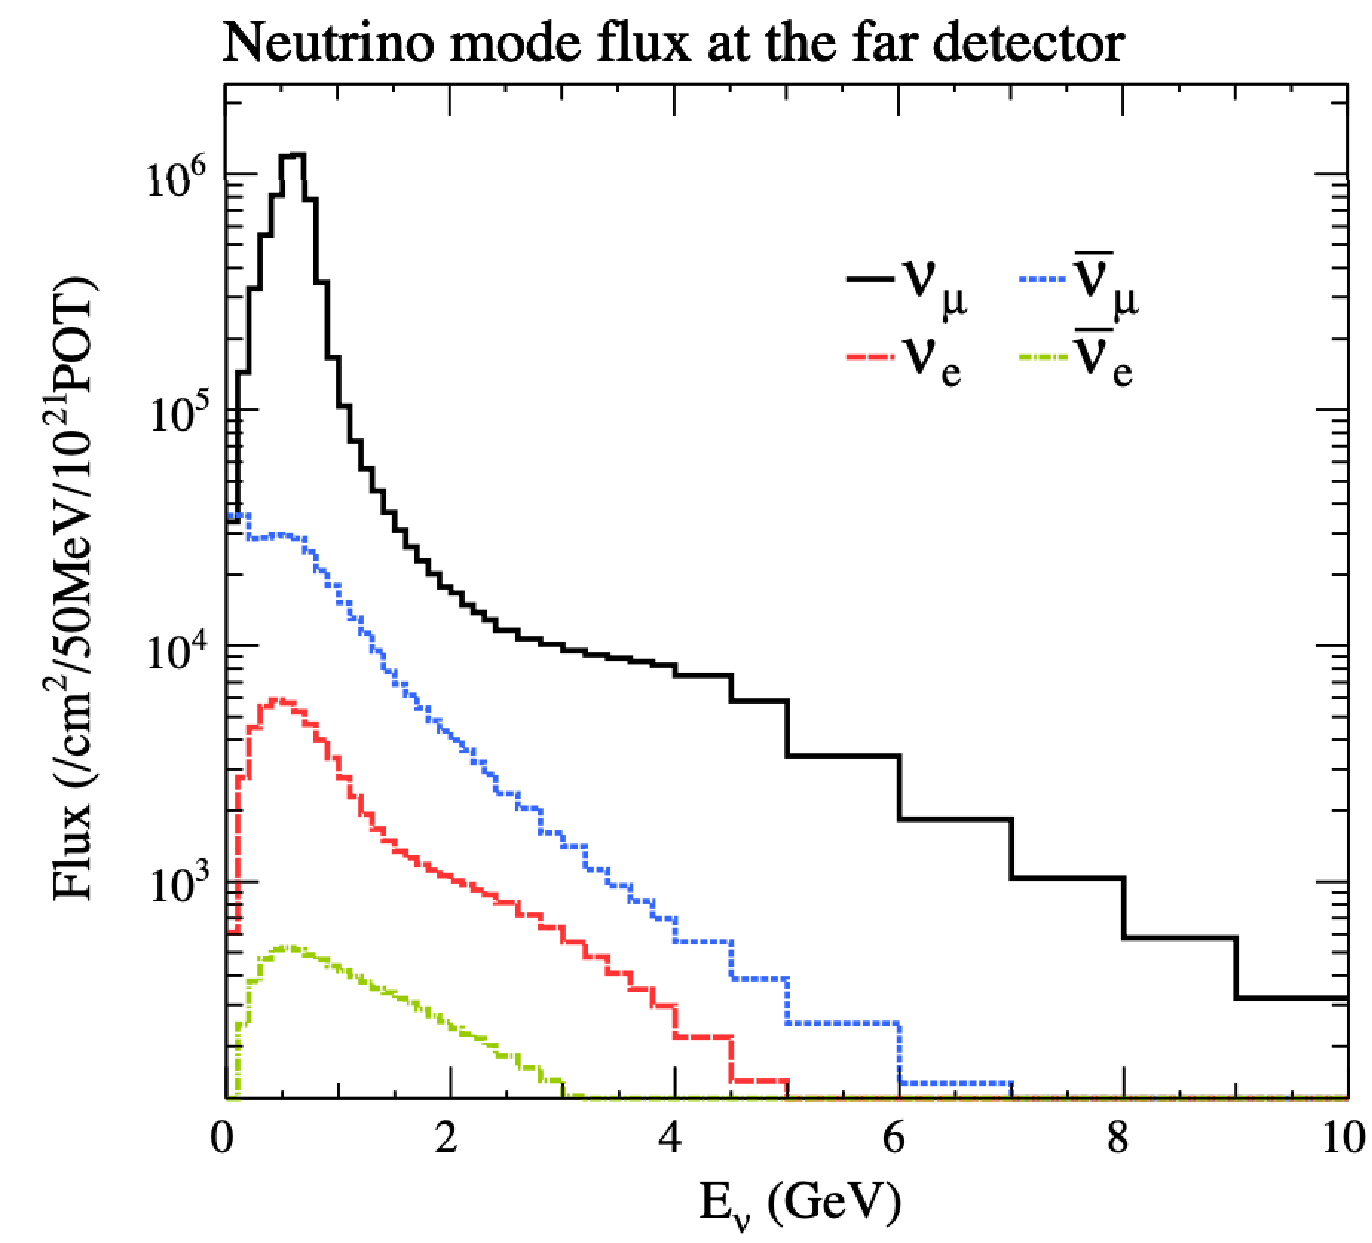
\includegraphics[width=\textwidth, trim={0mm 0mm 0mm 0mm}, clip,page=1]{Figures/Detectors/T2KFluxInNuMode.pdf}
  \end{subfigure}%
  \begin{subfigure}[t]{0.45\textwidth}
    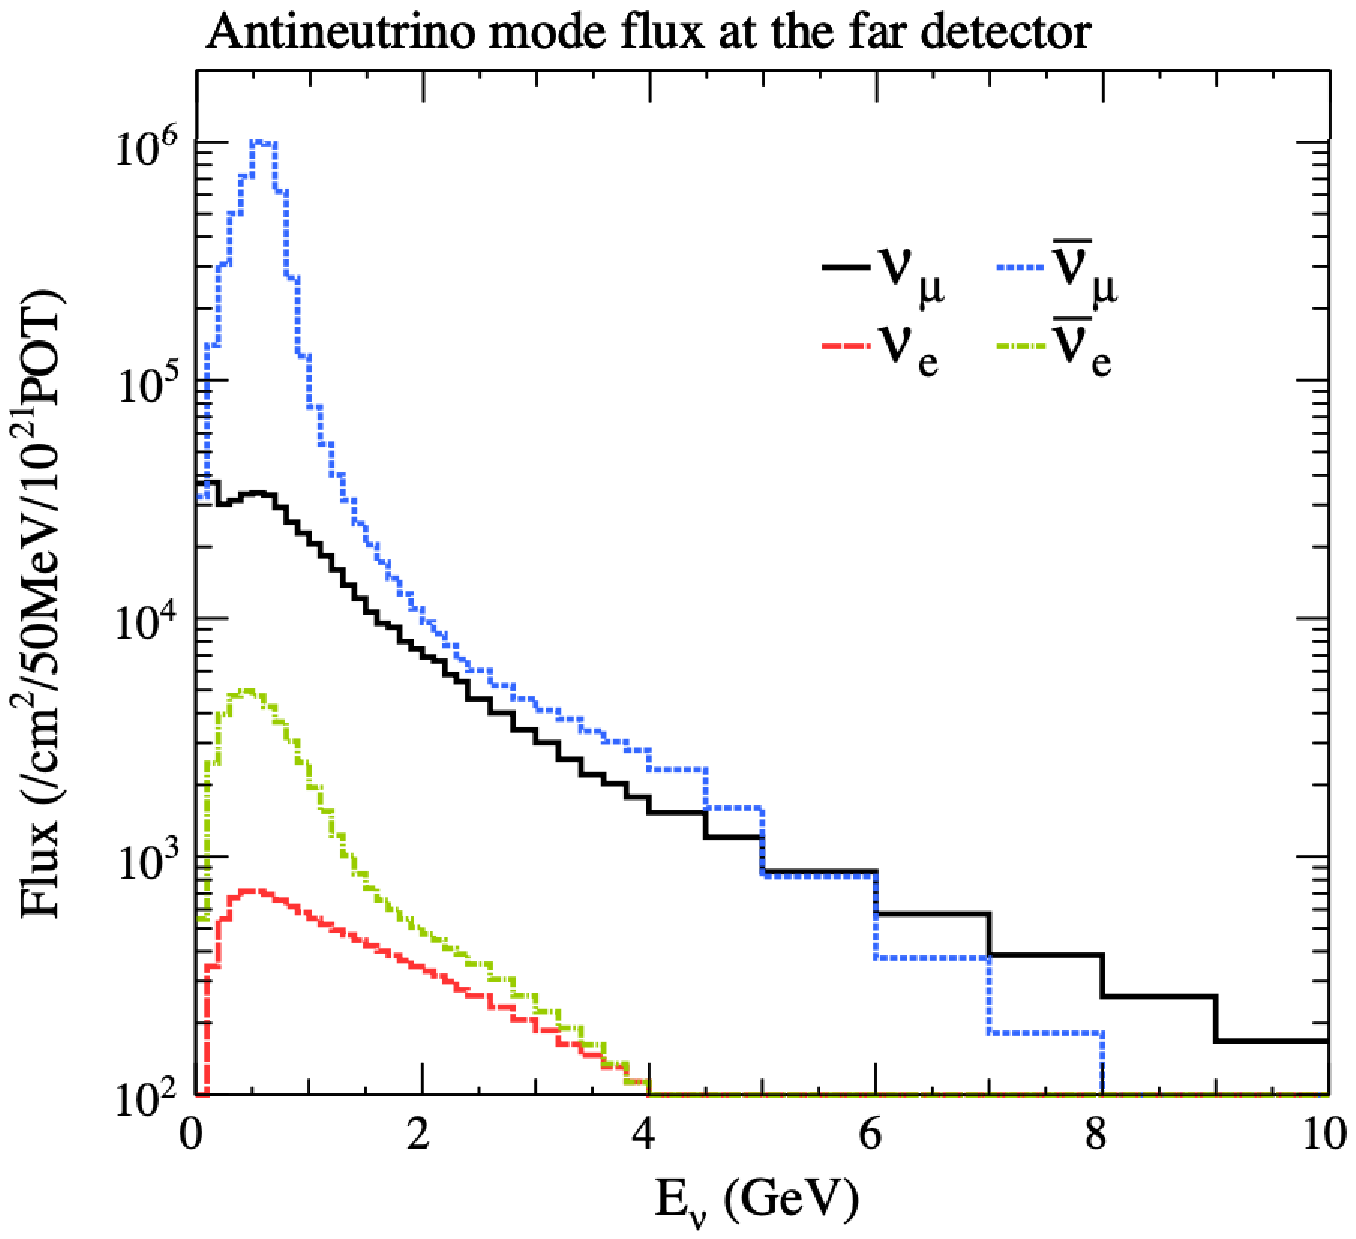
\includegraphics[width=\textwidth, trim={0mm 0mm 0mm 0mm}, clip,page=1]{Figures/Detectors/T2KFluxInANuMode.pdf}
  \end{subfigure}
  \caption{The energy spectrum for each flavour of neutrino (\quickmath{\nu/\bar{\nu}} and \quickmath{\nu_e/\nu_\mu}) in the neutrino dominated beam FHC mode (Left) and antirneutrino dominated beam RHC mode (Right) estimated by Monte Carlo. Taken from \cite{Abe2021-tr}.}
  \label{fig:T2KSKExp_T2K_NuFluxPerMode}
\end{figure}

The beam dump, situated at the end of the decay volume, stops all charged particles other than highly energetic muons (\quickmath{p_\mu > 5\text{GeV}}). The MuMon detector monitors the penentrating muons to determine the beam direction and intensity which is used to constrain some of the beam flux systematics within the analysis \cite{MuMon, Vladisavljevic2020-gv}. 

The T2K experiment uses the an off-axis beam to narrow the neutrino energy distribution. This was the first implementation of this technique in a long baseline neutrino oscillation experiment after its original proposal \cite{Beavis1995-qf}. Pion decay, \quickmath{\pi \rightarrow \mu + \nu_\mu}, is a two body decay. Consequently, the neutrino energy \quickmath{E_\nu} can be determined based on the pion energy, \quickmath{E_\pi} and the angle at which the neutrino is emitted, \quickmath{\theta},

\begin{equation}
  E_\nu = \frac{m^{2}_{\pi} - m^{2}_{\mu}}{2\left(E_\pi - p_\pi \cos(\theta) \right)},
\end{equation}

where \quickmath{m_{\pi}} and \quickmath{m_{\mu}} are the mass of the pion and muon respectively. Consequently, the neutrino eneregy distribution is dependent upon the angle at which the neutrinos are observed from the initial pion beam direction. For the \quickmath{295\text{km}} baseline at T2K, \quickmath{E_\nu = 0.6\text{GeV}} maximises the electron neutrino appearance probability, \quickmath{P(\nu_\mu \rightarrow \nu_e)}, whilst minimising the muon disappearance probability, \quickmath{P(\nu_\mu \rightarrow \nu_\mu)}. \autoref{fig:T2KSKExp_T2K_OffAxisTrick} illustrates the neutrino energy distribution for a range of off-axis angles, as well as the oscillation probabilities most relevant to T2K.

\begin{figure}[h]
  \begin{subfigure}[t]{0.7\textwidth}
    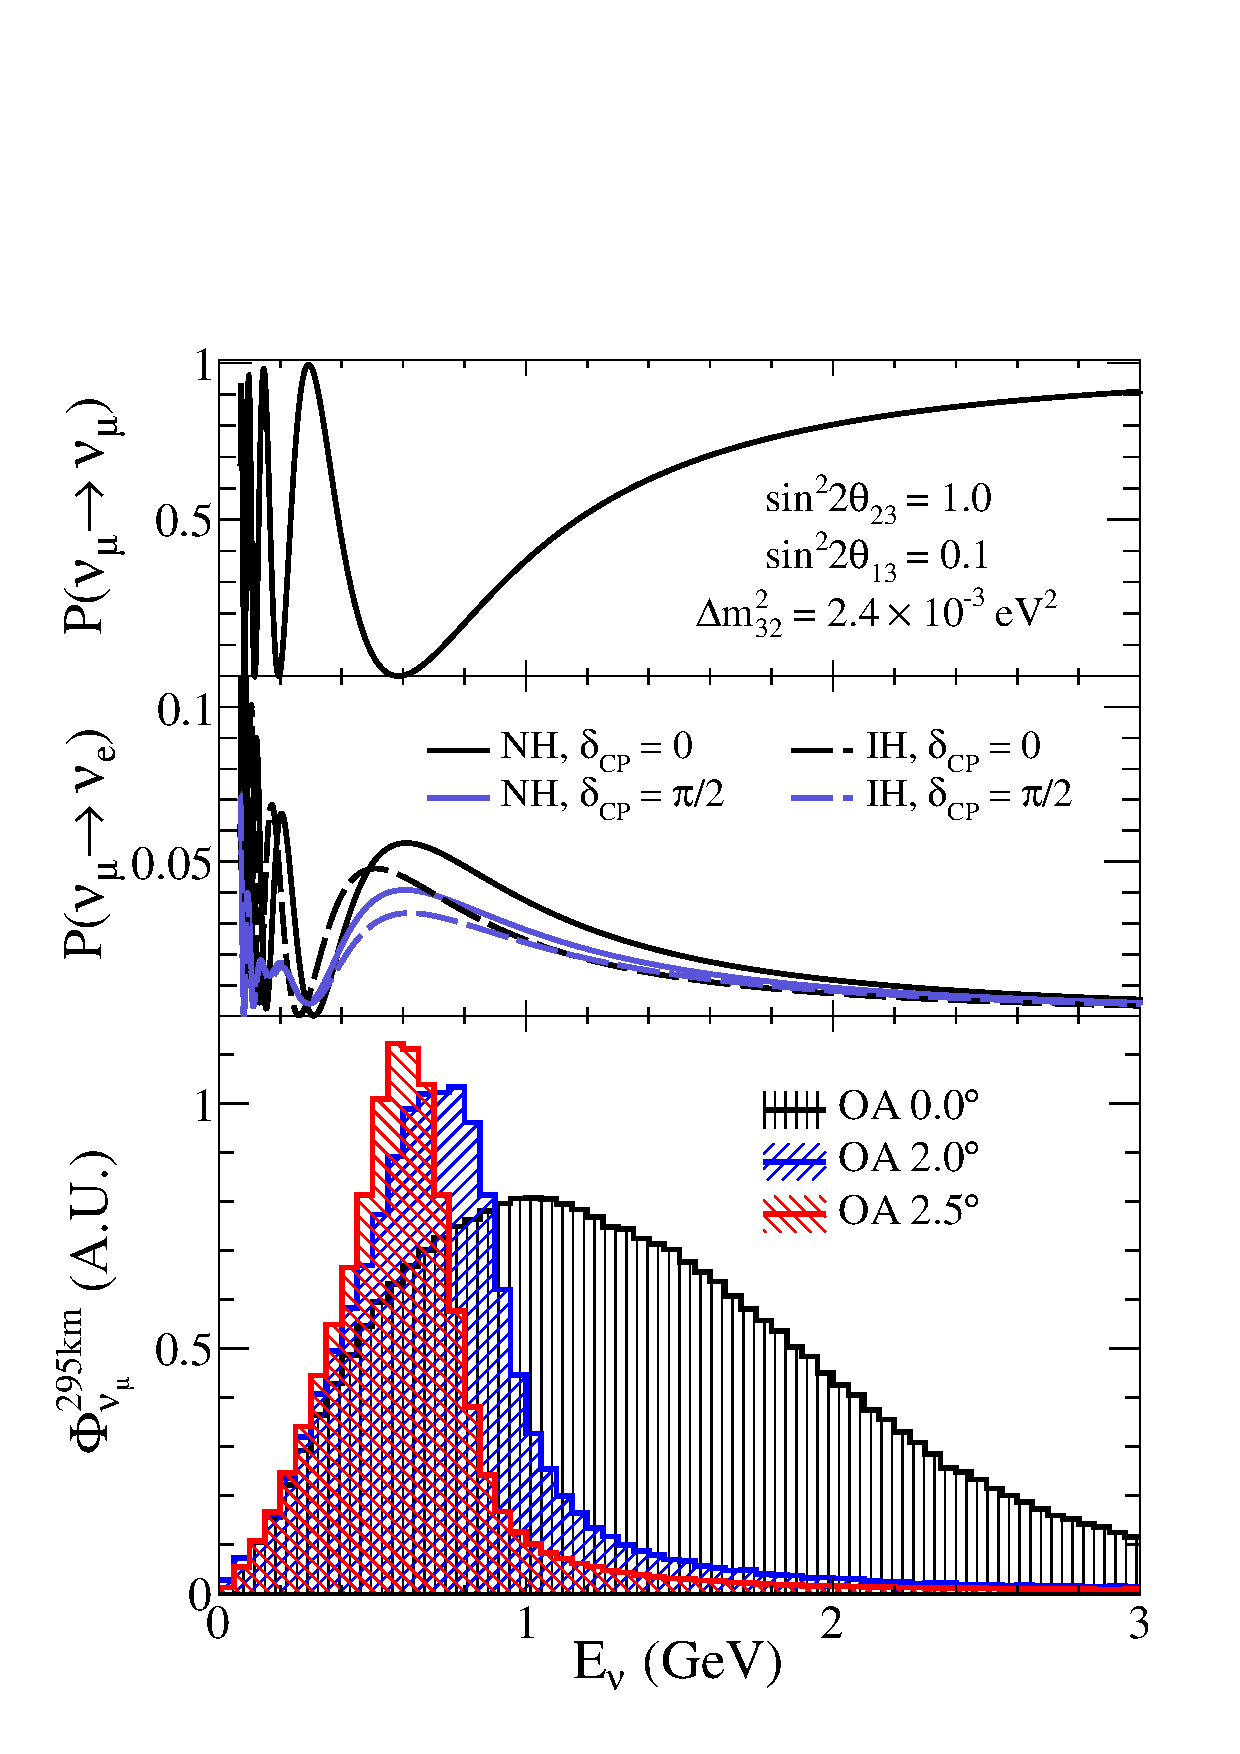
\includegraphics[width=\textwidth, trim={0mm 0mm 0mm 0mm}, clip,page=1]{Figures/Detectors/T2KOffAxisTrick.pdf}
  \end{subfigure}
    \caption{Top(Middle) panel: T2K muon neutrino disappearance(muon neutrino appearance) probability as a function of neutrino energy. Bottom panel: The neutrino energy distribution for three different off-axis angles (Arbitary units).}
  \label{fig:T2KSKExp_T2K_OffAxisTrick}
\end{figure}

\subsection{The Near Detector at \quickmath{280\text{m}}}
\label{subsec:T2KSKExp_T2K_ND280}

Whilst all the near detectors are situated in the same ``pit'' located at \quickmath{280\text{m}} from the beamline (as illustrated in \autoref{fig:T2KSKExp_T2K_ND280Pit}), the ``ND280'' detector is the off-axis detector which is situated at the same off-axis angle as the Super-Kamiokande far detector. It is designed to observe the unoscillated neutrino flux to measure the beam flux whilst also counting the event rate of the different interaction modes in which a neutrino can interact through. This allows the systematics used within the model to be constrained for a more accurate prediction of the expected event rate at the far detector.

\begin{figure}[h]
  \begin{subfigure}[t]{0.7\textwidth}
    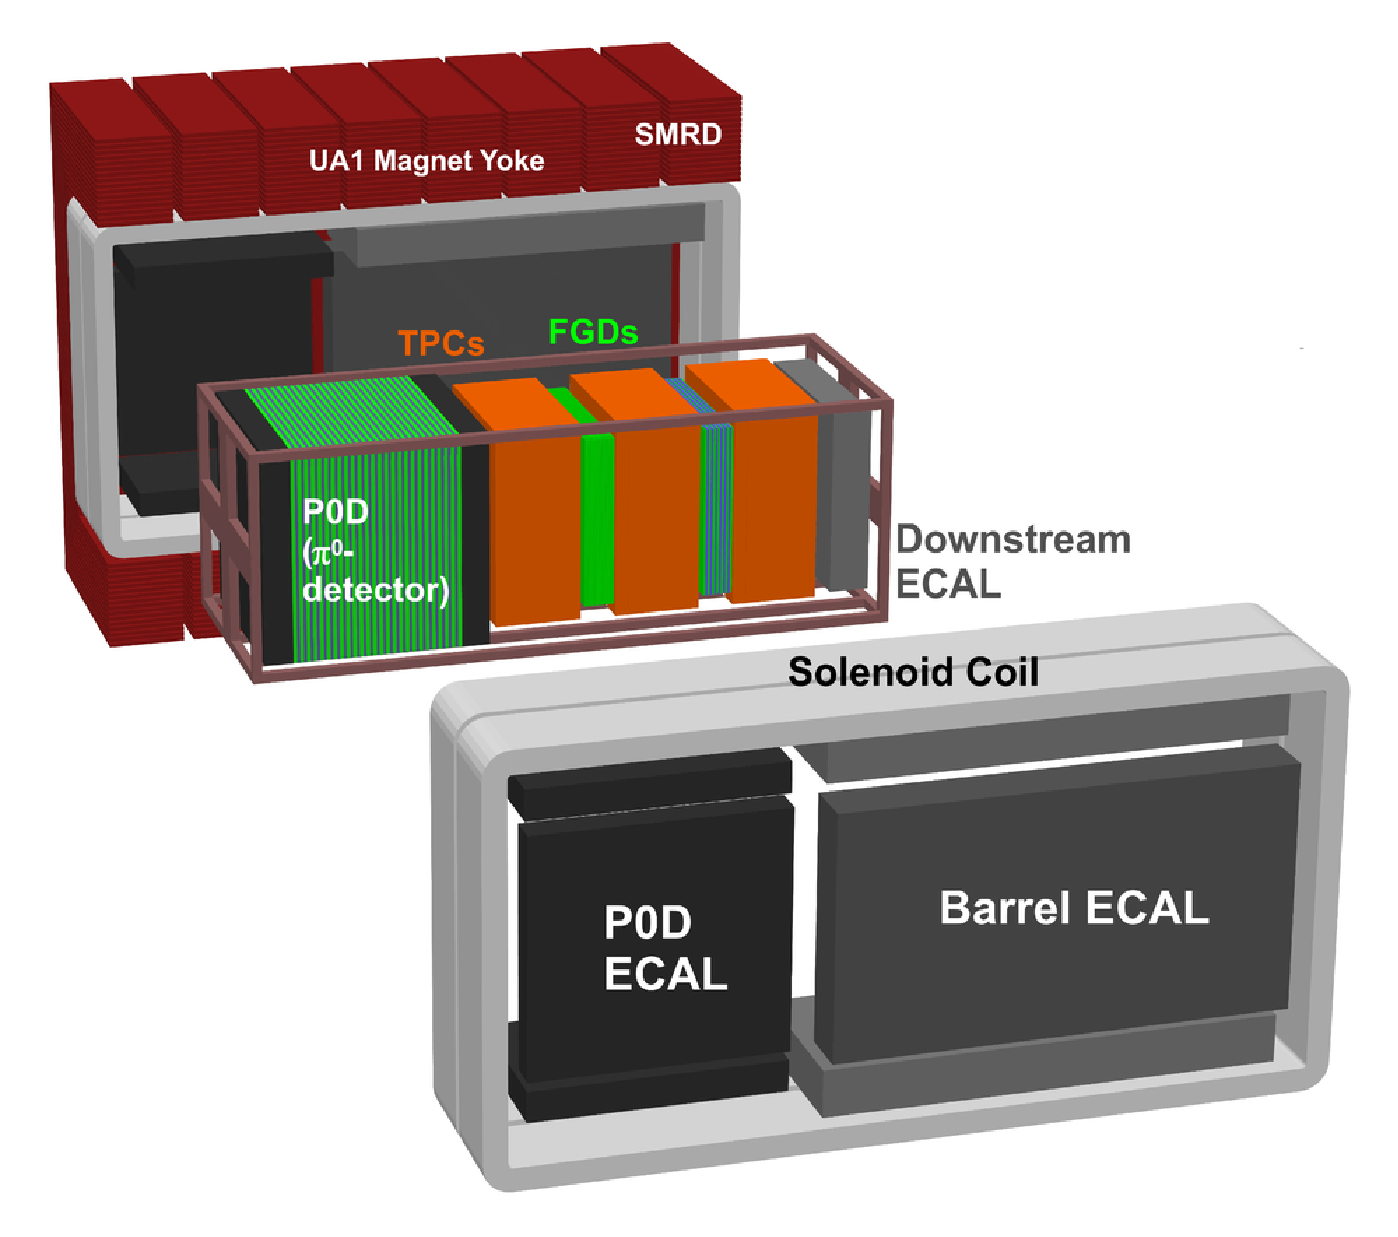
\includegraphics[width=\textwidth, trim={0mm 0mm 0mm 0mm}, clip,page=1]{Figures/Detectors/T2KND280.pdf}
  \end{subfigure}
    \caption{The components of the ND280 detector. The neutrino beam travels from right to left. Taken from \cite{t2k_det}.}
  \label{fig:T2KSKExp_T2K_ND280}
\end{figure}

As illustrated in \autoref{fig:T2KSKExp_T2K_ND280}, the ND280 detector is consists of several sub modules. The most important part of the detector for this analysis is the tracker region which is comprised of two time projection chambers (TPCs) sandwhiched beetween three fine grain detectors (FGDs). The FGDs contain both hydrocarbons and water targets for neutrino interactions and provide track reconstruction near the interaction vertex. The emitted charged particles can then propogate into the TPCs which provide particle identification and momentum reconstruction. The FPGs and TPCs are further described in \autoref{subsubsec:T2KSKExp_T2K_FGDs} and \autoref{subsubsec:T2KSKExp_T2K_TPCs} respectively. The electromagnetic calorimeter (ECAL) encapsulates the tracker region alongside the \quickmath{\pi^0} detector (P0D). The ECAL measures the deposited energy from photons emitted from interactions within the FGD and the P0D detector constrains the cross section of neutral current interactions which generate neutal pions, which are one of the largest backgrounds in the electron neutrino appearance oscillation channel. The P0D and ECAL detectors are detailed in \autoref{subsubsec:T2KSKExp_T2K_P0D} and \autoref{subsubsec:T2KSKExp_T2K_ECAL} respectively. The entire detector is located within a large yolk magnet which produces a \quickmath{0.2\text{T}} magnetic field. This design of the magnet also include a scintillating detector called the side muon range detector (SMRD) which is used to track high angle muons as well as acting as a cosmic veto. The SMRD is described in \autoref{subsubsec:T2KSKExp_T2K_SMRD}.  

\subsubsection{Fine Grained Detectors}
\label{subsubsec:T2KSKExp_T2K_FGDs}

The T2K tracker region is comprised of two fine grained detectors (FGD). The FGDs are the primary target material which are \quickmath{1.1} tonnes of target material per FDG for the neutrinos to interaction with. Alongside this, the FGDs are designed to be able to track short range particles which don't exit the particular FGD in which the neutrino interacted in. Typically, short range particles are low momentum which are observed as tracks which deposit a large amount of energy per unit length which means the FGD needs good granularity to resolve these particles. The FGDs have the best timing resolution (\quickmath{\sim 3\text{ns}}) of any of the sub-modules of the ND280 detector. As such, the FGDs are used for time of flight measurements to determine forward going positively charged particles from backward going negatively charged particles. Furthermore, the FGDs are used to temporarly tag tracks which pass through multiple sub-modules and any tracks which enter a TPC are required to be track-matched to a track found in the associated FGD.

Both FDGs are made from square scintillator planes of side length \quickmath{186\text{cm}} and width \quickmath{2.02\text{cm}}, which are made from two layers of 192 scintallator bars in an XY orientation. A wave-length shift fibre is threaded through the center of each bar and is readout by an multi-photon pixel counter (MPPC). FGD1 is the most upstream of the two FGDs and contains 15 planes of carbon plastic scintillator which is a common target in external neutrino scattering data. As the far detector is a pure water target, 7 of the 15 scintillator planes in FGD2 have been replaced with a hybrid water-scintillator target. Due to the complexity of the nucleus, nuclear effects can not be extrapolated between different nuclei.Therefore having the ability to take data on one target which is the same as external data and another target which is the same as the far detector target is benefical for reliable model parameter estimates.

\begin{figure}[h]
  \begin{subfigure}[t]{0.7\textwidth}
    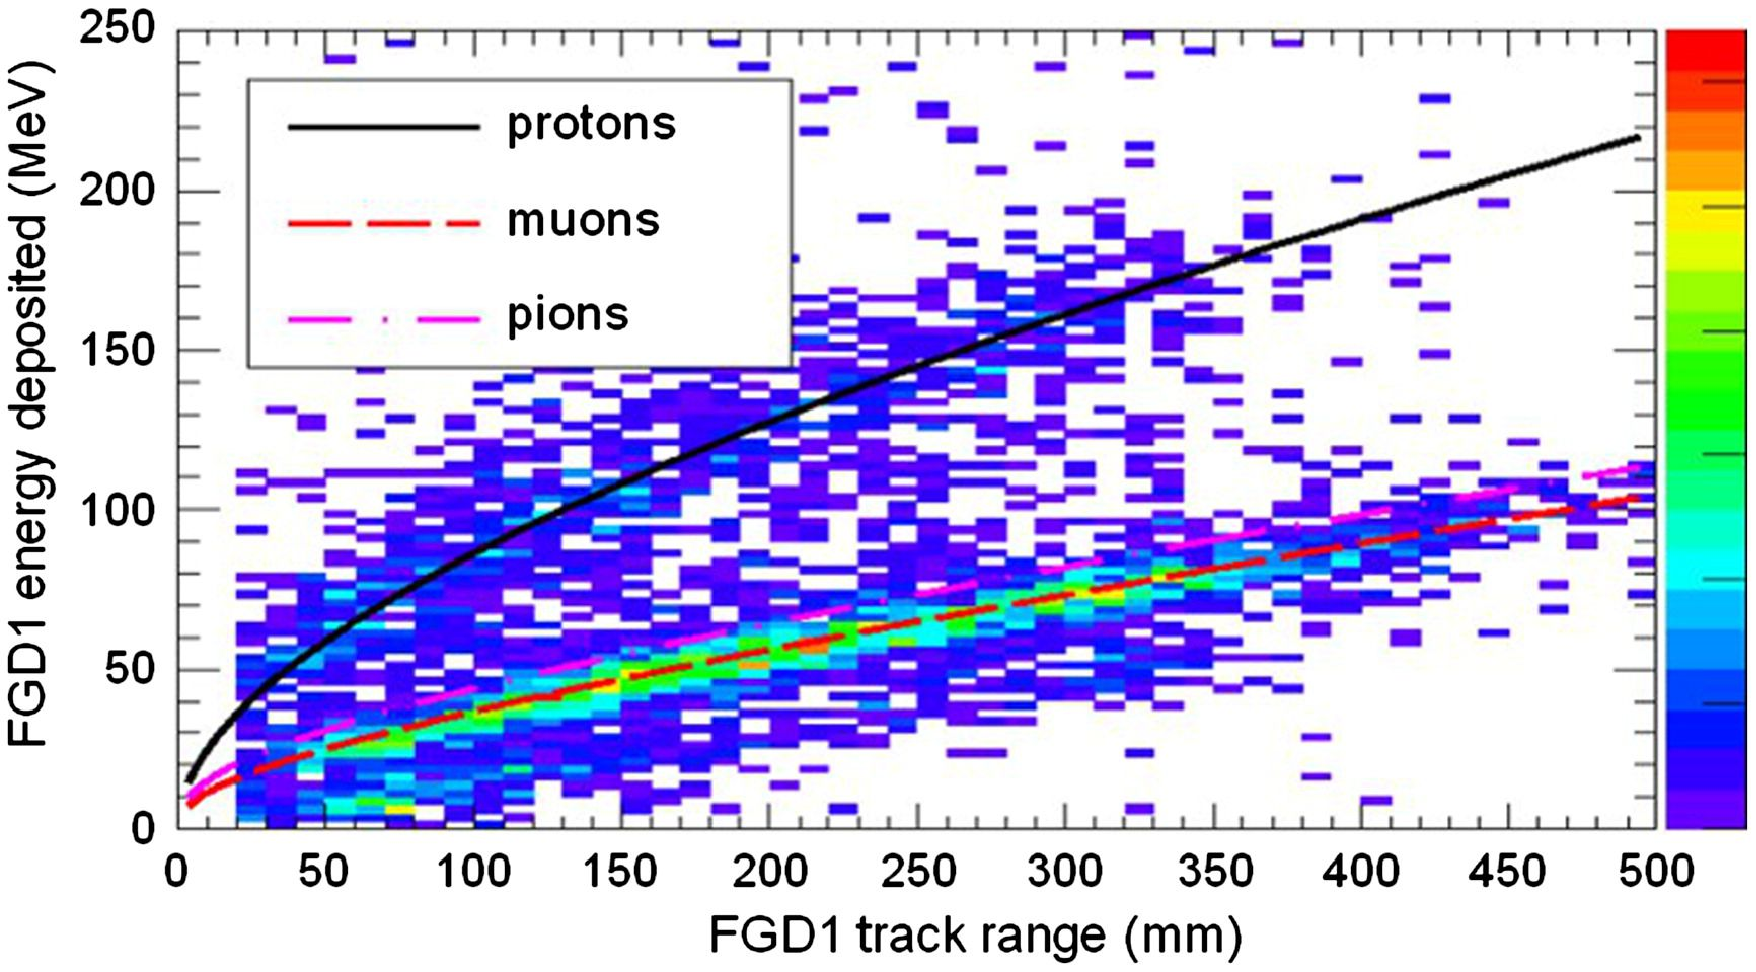
\includegraphics[width=\textwidth, trim={0mm 0mm 0mm 0mm}, clip,page=1]{Figures/Detectors/T2KFGDPID.pdf}
  \end{subfigure}
    \caption{Comparison of data to Monte Carlo prediction of integrated deposited energy as a function of track length for particles which stopped in FGD1. Taken from \cite{Amaudruz2012}.}
  \label{fig:T2KSKExp_T2K_FGDPID}
\end{figure}

For tracks which do not leave the FGD, the track lengths are often to small to make reliable dE/dx measurements. Consequently, the integrated deposited energy is used for particle identification. The FGD can distinguish protons from other charged particles by comparing the integratedd deposited energy from data to Monte Carlo prediction as seen in \autoref{fig:T2KSKExp_T2K_FGDPID} for particles stopping in FDG1.

\subsubsection{Time Projection Chambers}
\label{subsubsec:T2KSKExp_T2K_TPCs}

\subsubsection{\quickmath{\pi^0} Detector}
\label{subsubsec:T2KSKExp_T2K_P0D}

\subsubsection{Electromagnetic Calorimeter}
\label{subsubsec:T2KSKExp_T2K_ECAL}

\subsubsection{Side Muon Range Detector}
\label{subsubsec:T2KSKExp_T2K_SMRD}

\subsection{The Interactive Neutrino GRID}
\label{subsec:T2KSKExp_T2K_INGRID}

The Interactive Neutrino GRID (INGRID) detector is situated within the same ``pit'' as the other near detectors and is aligned with the beam in the ``on-axis'' position. It is designed to measure the beam direction, spread and intensity. The detector was originally designed with 16 identical modulues \cite{t2k_det} (two modules have since been switched off) and a ``proton'' module. The design of the detector is cross-shaped with length and height \quickmath{10\text{m} \times 10\text{m}} as illustrated in \autoref{fig:T2KSKExp_T2K_INGRID}. Each module is composed of iron sheets interlaced with eleven tracking scintillator planes for a total target mass of \quickmath{7.1} tonnes. The scintillator design is an X-Y pattern of 24 bars in both orientations, where each bar contains wave-length shifting fibres which are connected to multi-pixel photon counters (MPPCs). The MPPCs convert detected photons into electrical signals via photodiodes which is then readout by Trip-T front-end electronics \cite{Yokoyama2010} and passed to the readout merging modules along with timing information from the clock module. Each module is encapuslated with veto plates to aide rejection of charged particles entering the module.

The proton module is different from the other modules in that it consists of entirely scintillator planes with no iron target. The scintillator bars are also smaller than those used in the other modules to increase the granularity of the detector and improve tracking capabilities. The module sits in the center of the beamline and is designed to give precise measurments of quasi-elastic charged current interactions to evaluate the performance of the monte carlo simulation of the beamline. 

\begin{figure}[h]
  \begin{subfigure}[t]{0.45\textwidth}
    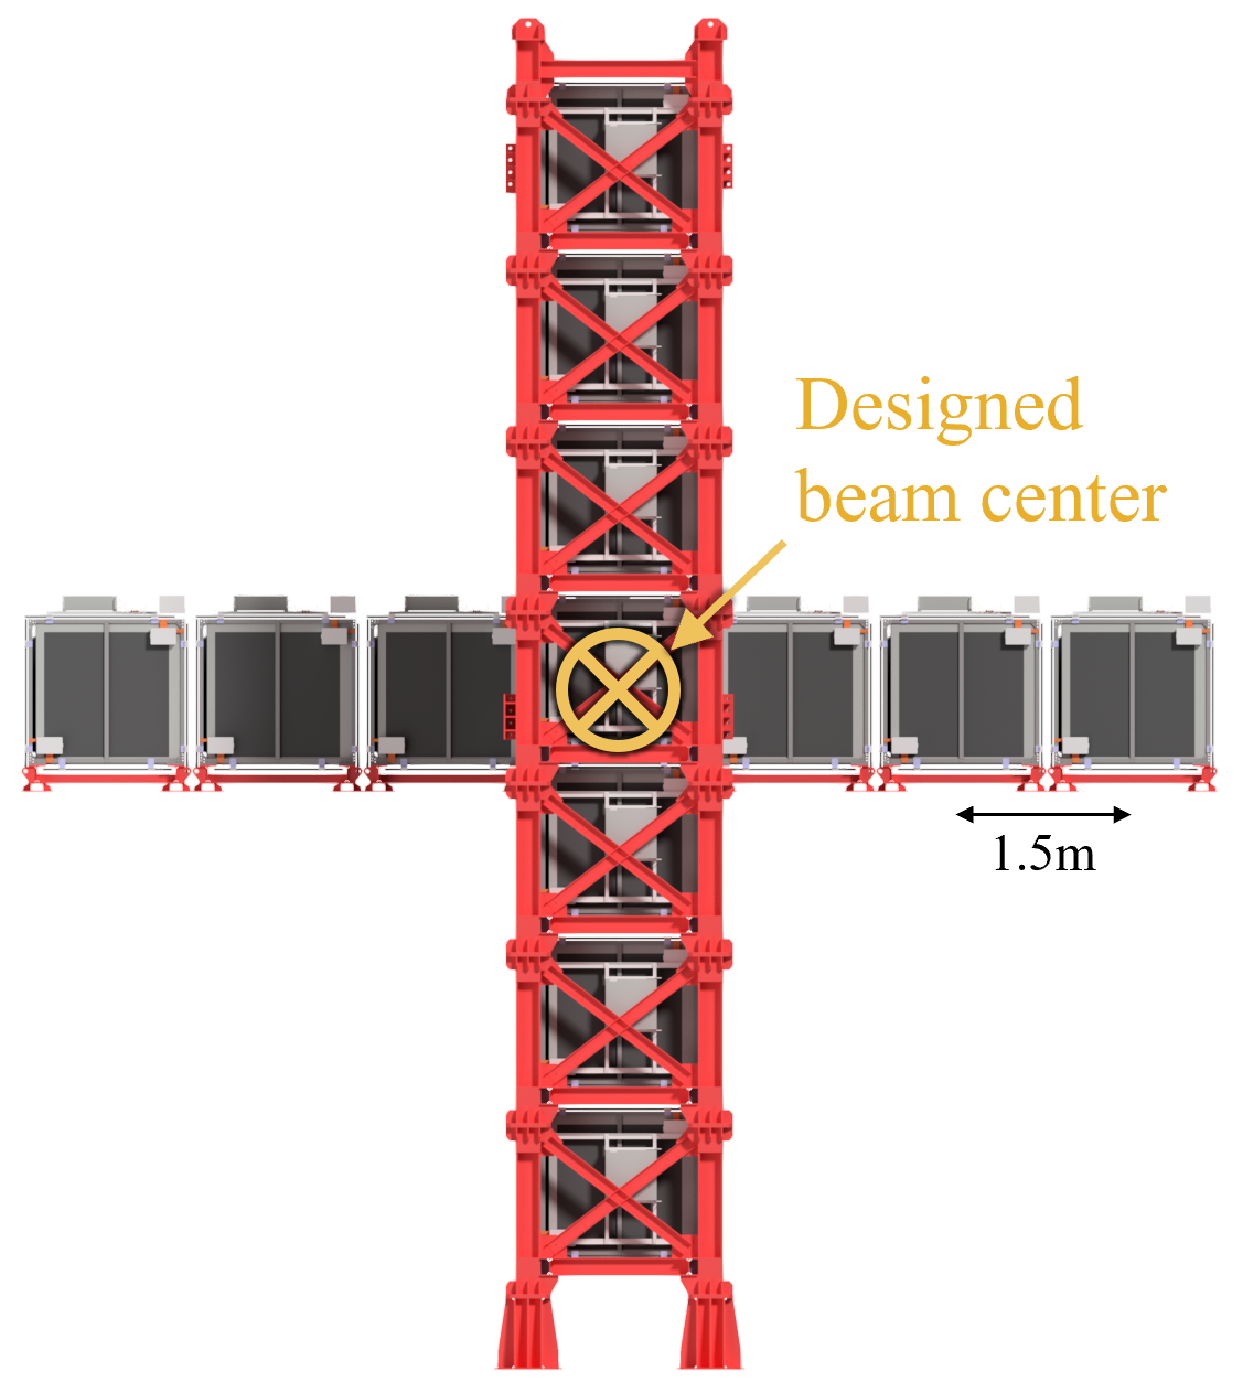
\includegraphics[width=\textwidth, trim={0mm 0mm 0mm 0mm}, clip,page=1]{Figures/Detectors/T2KINGRIDDiagram.pdf}
  \end{subfigure}%
  \begin{subfigure}[t]{0.55\textwidth}
    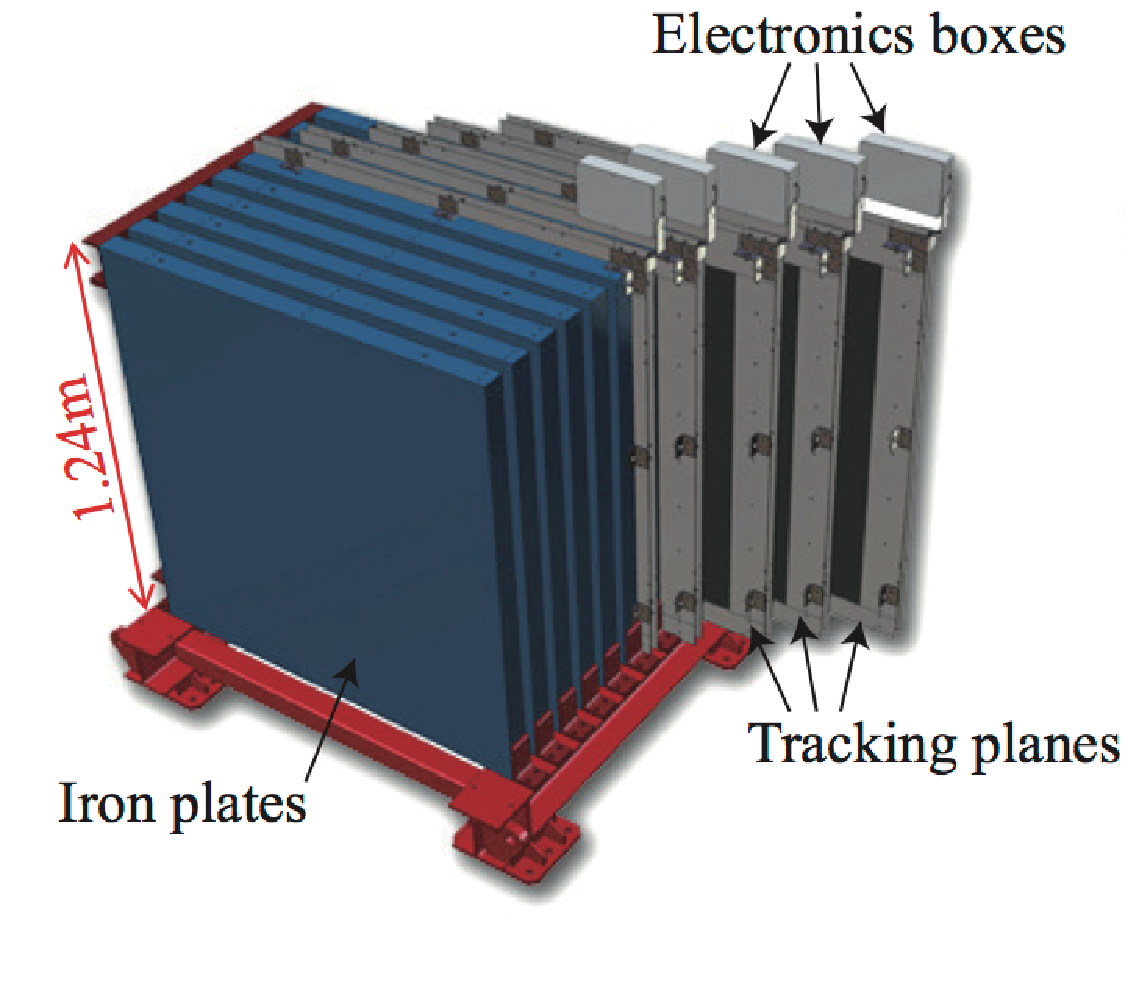
\includegraphics[width=\textwidth, trim={0mm 0mm 0mm 0mm}, clip,page=1]{Figures/Detectors/T2KINGRIDModule.pdf}
  \end{subfigure}%
  \caption{Left panel: The Interactive Neutrino GRID on-axis Detector. 14 modules are arranged in a cross shape configuration, with the centre modules being directly aligned with the on-axis beam. Right panel: The layout of a single module of the INGRID detector. Both figures recreated from \cite{t2k_det}.}
  \label{fig:T2KSKExp_T2K_INGRID}
\end{figure}

The INGRID detector can measure the beam direction to an uncertainty of \quickmath{0.4\text{mrad}} and the beam center within a resolution of \quickmath{10 \text{cm}} \cite{t2k_det}. The beam direction in both the vertical and horizontal directions is discussed in \cite{Suzuki_2015} and it is found to be in good agreement with the MUMON monitor described in \autoref{subsec:T2KSKExp_T2K_NeutrinoBeam}.


